%%%
% Page limit: 6 pages, + 1 page references
%Todo
% 
% for presentation
% 1. \footnote{\textbf{Sajjad} would be nice to have one diagram for our running example where we show the empty graph, the complete graph, and the intermediate graph learned by the normalized gain.} 
\documentclass{article}
\usepackage{ijcai17}
\usepackage{times}
%Preamble File for Tutorial

\usepackage{times}
\usepackage{graphicx}
\graphicspath{{../../}{figures/}}
%Theorems and such

%\usepackage{amsthm}

\newtheorem{theorem}{Theorem}
%\newtheorem{observation}{Observation}
\newtheorem{proposition}{Proposition}
\newtheorem{definition}{Definition}

%\usepackage{proceed2e}
%\usepackage{ltexpprt}
% defines theorem environments etc.


%\newtheorem{theorem}{Theorem}[section]
\newtheorem{observation}{Observation}[section]
\newtheorem{hypo}{Hypotheses}[section]
%\newtheorem{proposition}{Proposition}[section]
%\newtheorem{definition}{Definition}[section]

%%%%%%%%%%%%%%%%%%
% Packages
%%%%%%%%%%%%%%%%%%

\usepackage[ruled,vlined]{algorithm2e}
\usepackage{algorithmic}
%\usepackage{amsthm}
\usepackage{amsmath}
\usepackage{amsfonts}
\usepackage{amssymb}
\usepackage{graphicx}
\usepackage{url}
\usepackage{subfigure}
\usepackage{epstopdf}
%\setcounter{MaxMatrixCols}{30}
\usepackage{multirow}
\usepackage{subfigure}
\usepackage{ifthen}
\DeclareMathOperator*{\argmax}{argmax}
\DeclareMathOperator*{\argmin}{argmin}
\DeclareMathOperator{\NP}{\mathbf{\mathrm{NP}}}

%%%%%%%%%%%%%%%%%%%%
% font styles
%%%%%%%%%%%%%%%%%%

\def\defterm#1{\textbf{#1}}
%\def\set#1{\mathbf{#1}}
\def\set#1{\bs{#1}}
\def\bs#1{\boldsymbol{#1}}
\def\ground#1{\overline{#1}}


%%%%%%%
% values
%%%%%%%

\newcommand{\male}{M}
%%%%%%%%
% other systems

\newcommand{\foil}{\textsc{FOIL}}
%%%%%%%%%%%%%%%%%%%
% relational structures
%%%%%%%%%%%%%%%%%%

\newcommand{\structure}{w}
\newcommand{\individuals}{\mathcal{I}}
\newcommand{\functors}{\mathcal{F}}\newcommand{\values}{\mathcal{V}}
\newcommand{\samplesize}{N}
\newcommand{\psize}[2]{N\left[#1;#2\right]}
%usage{\psize{population}{dstructure}
\newcommand{\varsize}[2]{\psize{#1}{#2}}
%usage \varsize{pvariable}{dstructure}
%%%%%%%%%
% special functors


% for population variables
\newcommand{\Avariable}{\mathbb{A}}
\newcommand{\Bvariable}{\mathbb{B}}
\newcommand{\Cvariable}{\mathbb{C}}
\newcommand{\Uvariable}{\mathbb{U}}

%for individual constants
\newcommand{\aconstant}{a}
\newcommand{\bconstant}{b}
\newcommand{\cconstant}{c}

% for classes, sorts, types

\def\varclass#1#2{#1_{#2}}
%usage \varclass{\individuals}{\Avariable}


% for functors

\newcommand{\functor}{f}
\newcommand{\Ppredicate}{P}
\newcommand{\Rpredicate}{R}
\newcommand{\class}{\it{Class}}
% for functors representing classes
\newcommand{\indclass}{\individuals}
\newcommand{\relationship}{\it{Relation}}
% for functors representing classes

% various constants
\newcommand{\true}{\mathrm{T}}
\newcommand{\false}{\mathrm{F}}
\newcommand{\na}{\it{na}}
\newcommand{\normalconstant}{Z} % the normalization constant

%formulas and such
%first-order variables
\newcommand{\Xvariable}{X}
\newcommand{\Yvariable}{Y}
\newcommand{\numvalues}[1]{r_{#1}}
% usage \numvalues{i}
%terms and compounds
\newcommand{\term}{\tau}
\def\fterm#1#2{#1(#2)}
%usage \term{\functor}{\terms}
\newcommand{\literal}{l}
\newcommand{\conjunction}{C}
\newcommand{\formula}{\phi}
\newcommand{\numformulas}{m}

%%%%%%%%%%%%%%%%%%
% Groundings
%%%%%%%%%%%%%%
\def\FG#1{#1^{\ast}}
\newcommand{\grounding}{\gamma}
\def\groundnode#1{\gamma_{#1}}
\def\replace#1#2{#1\backslash#2}
% \replace{population variable \textbackslash constant
\def\ground#1#2{\FG{#1}_{#2}}
%usage: \groundobject{object}{grounding}
\def\instantiate#1#2{#1_{#2}}
\def\groundall#1{\Gamma_{#1}}
% \groundall{Gamma}{set of pvariables}
%the substitution space of a set of variables

\def\resultset#1#2{\mathcal{R}_{#1}(#2)}
%usage \resultset{structure}{formula}

% Annotations marking degree of grounding
\newcommand{\UG}[2][0.0ex]{#2^{-}\hspace{#1}}
\newcommand{\PG}[2][0.0ex]{#2^{\prime}\hspace{#1}}
%\newcommand{\FG}[2][0.0ex]{#2^{*}\hspace{#1}}


%%%%%%%%%%%%%%%%
% Counts and probabilities
%%%%%%%%%%%%%%%%

\newcommand{\dset}{D}
\newcommand{\dstructure}{\mathcal{D}}
% observed substructure
\def\dminus#1#2{\FG{#1}_{-#2}}
%usage: \dminus{dstructure}{ground atom}
%\def\dvalues#1#2#3{#1_{#2}(#3)}
%%observed values in D. usage: dvalues{values}{variables}{Database}
\def\dvalues#1#2#3{#1^{#2}_{#3}}
%observed values in D. usage: dvalues{varvalue}{grounding}{Database}
\def\dprob#1#2{P_{#1}(#2)}

%%%%%%%%%
% deprecate these
\def\dlog#1#2{L_{#1}(#2)}
% usage: dprob{structure}{formula}
\def\dlogcount#1#2#3{L^{#1}_{#2}(#3)}
% usage: L{model}{node index}{database}
\def\dlogfreq#1#2#3{\nscore{L}^{#1}_{#2}(#3)}
% usage: L{model}{node index}{database}
\def\aiclocal#1#2#3{\it{AIC}^{#1}_{#2}(#3)}
% usage: AIC{model}{node index}{database}
\def\aicfreq#1#2#3{\nscore{\it{AIC}}^{#1}_{#2}(#3)}
% usage: AIC{model}{node index}{database}
\def\biclocal#1#2#3{\it{BIC}^{#1}_{#2}(#3)}
% usage: BIC{model}{node index}{database}


\def\spenalty#1#2#3#4{f^{#1}(\numpars{#3}{#2},#4)}
%usage \spenalty{scorename}{node index}{graph}{countvector}

\def\numpars#1#2{\#\it{pars}_{#2}(#1)}
% usage \numpars{\BN}{i}

\def\Score#1#2#3{#1(#2,#3)}
%usage \Score{scorename}{\BN}{\D}
\def\score#1#2#3#4{#1_{#2}(#3,#4)}
%\def\score#1#2#3#4{#1_{#3}(#2,#4)}
% usage: \score{scorename}{node index}{graph}{database}
% usage: \score{scorename}{node index}{parents}{database}
%\def\gain#1#2#3#4#5{\improve{#1}_{#4}(#2,#3',#5)}
\def\Gain#1#2#3#4{#1(#2,#3,#4)}
%usage \Gain{gainname}{\BN}{\BN'}{dstructure}
\def\gain#1#2#3#4{#1_{#2}(#3,#3^{+},#4)}
% usage: \gain{scorename}{node index}{model}{database}
\newcommand\parloss[2]{\improve{\it{pars}}({\node_{i},{\Parents{#1}{#2},\node_{+}}})}
%usage: parloss{node index}{model}
%score names


\newcommand{\loglikelihood}{LL}
\newcommand{\aic}{AIC}
\newcommand{\bic}{BIC}
\newcommand{\bdeu}{BDeu}
\newcommand{\rescale}{\loglikelihood_{\it{scale}}}

\def\cscore#1{#1}
%count score
\def\nscore#1{\overline{#1}}
%\def\nscore#1{#1}
% normalized score
\def\ncscore#1{\widetilde{#1}}
%\def\gain#1{\overline{#1}}
\def\improve#1{\Delta#1}
\def\logimprove#1#2#3#4{\improve{L}^{#1,#2}_{#3}(#4)}
%usage \logimprove{BN1}{BN2}{i}{dstructure}
\def\flogimprove#1#2#3#4{\improve{\nscore{L}}^{#1,#2}_{#3}(#4)}
%usage \logimprove{BN1}{BN2}{i}{dstructure}
\def\aicimprove#1#2#3#4{\improve{\nscore{\it{AIC}}}^{#1,#2}_{#3}(#4)}
\def\bicimprove#1#2#3#4{\improve{\nscore{\it{BIC}}}^{#1,#2}_{#3}(#4)}

\def\rlog#1#2{\Relevant{L}_{#1}(#2)}
\def\bprob#1#2#3{#1_{#2}(#3)}
% usage: bprob{P}{BN}{assignment}
\def\iprob#1{\FG{P}(#1)}
% usage iprob{ground formula/term}
\newcommand{\probworlds}{\mu}
%distribution over structures


%%%%%%%%%%%%
%DB counts
%%%%%%%%%

\newcommand{\Cvar}{\mathrm{n}}
\newcommand{\Fvar}{\mathrm{p}}
\newcommand{\Relevant}[1]{#1^{\mathrm{r}}}
\newcommand{\relevant}[1]{\it{R}_{#1}}
%usage \relevant{index}

\newcommand{\Count}[2]{\Cvar\left[#1;#2\right]}
%e.g.n[formula;database]
\newcommand{\Fcount}[3]{\Cvar^{#1}_{#2}(#3)}
%usage \fcount{\bn}{ijk}{dstructure}
\newcommand{\Fbcount}[3]{\set{\Cvar}^{#1}_{#2}(#3)}
\newcommand{\Fpcount}[3]{\overline{\set{\Cvar}}^{#1}_{#2}(#3)}
\newcommand{\Rcount}[3]{\Relevant{\Cvar}\left[{#1};#2\right]}
%usage \Rcount{formula}{dstructure}
\newcommand{\Frcount}[3]{\Relevant{\Cvar}_{#1}(#2)}
%usage \Rcount{ijk}{dstructure}
\newcommand{\countvec}[3]{\set{\Cvar}^{#1}_{#2}(#3)}
%usage \countvec{countvector symbol}{graph}{data}


\newcommand{\Freq}[2]{\Fvar\left[#1;#2\right]}
%e.g.n[formula;database]
\newcommand{\Ffreq}[2]{\Fvar_{#1}(#2)}
%usage \ffreq{ijk}{dstructure}
\newcommand{\Rfreq}[2]{\Relevant{\Fvar}\left[{#1};#2\right]}
%usage \Rfreq{formula}{dstructure}
\newcommand{\Frfreq}[2]{\Relevant{\Fvar}_{#1}(#2)}
%usage \Rfreq{ijk}{partial grounding}{dstructure}


%\newcommand{\Freq}[2]{\Fvar\left[#1;#2\right]}
%%e.g.n[formula;database]
%\newcommand{\Rfreq}[2]{\Relevant{\Fvar}\left[#1;#2\right]}
%\newcommand{\Ffreq}[2]{\Fvar_{#1}(#2)}
%%usage \fcount{ijk}{dstructure}
%\newcommand{\Frfreq}[2]{\Relevant{\Fvar}_{#1}(#2)}

%


%\newcommand{\Count}[2]{#1(#2)}
%%count of database
%%usage \bncount{\Cvar_{ijk}}{dstructure}
%\newcommand{\CountC}[2]{\Cvar_{ijk}\left[#1;#2\right]} %count in database satisfying grounding

%\newcommand{\drcount}[1]{\Relevant{\Cvar}_{ijk}\left[#1\right]}
%%count of database
%\newcommand{\drcountC}[2]{\Relevant{\Cvar}_{ijk}\left[#1;#2\right]} %count in database satisfying grounding
%
%\newcommand{\dfreq}[2]{#1(#2)}
%%frequency database
%\newcommand{\dfreqC}[2]{\Fvar_{ijk}\left[#1;#2\right]} %frequency in database satisfying grounding
%\newcommand{\drfreq}[1]{\Relevant{\Fvar}_{ijk}\left[#1\right]}
%%frequency in database
%\newcommand{\drfreqC}[2]{\Relevant{\Fvar}_{ijk}\left[#1;#2\right]} %frequency in database satisfying grounding



%%%%%%%%%%%%%%%%%%%%%%
% Bayesian networks
%%%%%%%%%%%%%%%%



% Functions for graph structure
\newcommand{\BN}{B}
\newcommand{\mln}{M}
\newcommand{\node}{\Xvariable}
\newcommand{\graph}{G}
\newcommand{\MB}[1]{\mathrm{MB}(#1)}
\newcommand{\bnparents}{\mathrm{Pa}}
\newcommand{\Parents}[2]{\mathrm{Pa}_{#1}^{#2}}
%usage \Parents{\nodeindex}{\model}
\newcommand{\pavalue}[2]{\mathbf{pa}_{#1}^{#2}}
%usage \pavalue{i}
\newcommand{\numparents}[2]{q_{#1}^{#2}}
% usage \numparents{i}{\graph}
\def\numpars#1#2{\#\it{pars}_{#2}^{#1}}
% usage \numpars{\BN}{i}
\newcommand{\Ch}[1]{\mathrm{Ch}(#1)}
\newcommand{\nodevalue}{\it{v}}
\newcommand{\xvalue}{x}
\newcommand{\yvalue}{y}
%\newcommand{\parent}{\mathit{pa}}


\newcommand{\parameter}{\theta}
% Key functions for parameters
\newcommand{\w}{w}
\newcommand{\mprob}[2]{#1(#2)}
% usage \mprob{P}{node_{i = value k}}
%marginal probability
\newcommand{\cprob}[3]{#1(#2|#3)}
%usage \cprob{P}{x}{y}
\newcommand{\estcprob}[1]{\widehat{\parameter}_{ijk}(#1)}
%usage \estcprob(\dstructure)


\newcommand{\family}[2]{#1^{#2}}
%usage: \family{\node}{i}
\newcommand{\familyvalue}[1]{\xvalue_{#1}}
%usage: \familyvalue{ijk}
\newcommand{\familyf}[2]{(\node_{#1},\Parents{\node_{#1}})=\xvalue_{#2}}
%% usage: \familyf{i}{ijk}

%%%%%%%%%%%%%%
%
% conditional probabilities in log-linear model

\newcommand{\Gpvar}{\FG{P}}
\newcommand{\Gprob}[2]{\Gpvar(#1 | #2)}







\usepackage{amssymb}
\usepackage{graphicx}
\usepackage[small]{caption}
%\usepackage{subcaption}

\usepackage{url}


\title{Locally Consistent Bayesian Network Scores for Multi-Relational Data\thanks{Supported by a Discovery Grant from the Natural Sciences and Engineering Research Council of Canada. We thank Mark Schmidt and Leonid Chindelevitch for helpful suggestions.}}

\author{Oliver Schulte and Sajjad Gholami\\ 
Simon Fraser University, Burnaby, Canada\\
\{oschulte,sgholami\}@cs.sfu.ca}

\begin{document}

\maketitle

%\bibliographystyle{abbrv}

%\title{Outline for a Paper}
%\author{Oliver Schulte\\
%\\ School of Computing Science\\ Simon Fraser University\\Vancouver-Burnaby, Canada}
%\date{\today}
%\mainmatter  % start of an individual contribution

% first the title is needed
%\title{Upgrading Bayesian Network Scores for Multi-Relational Data}

% a short form should be given in case it is too long for the running head
%\titlerunning{Bayesian Network Scores for Multi-Relational Data}

% the name(s) of the author(s) follow(s) next
%
% NB: Chinese authors should write their first names(s) in front of
% their surnames. This ensures that the names appear correctly in
% the running heads and the author index.
%


%
% NB: a more complex sample for affiliations and the mapping to the
% corresponding authors can be found in the file "llncs.dem"
% (search for the string "\mainmatter" where a contribution starts).
% "llncs.dem" accompanies the document class "llncs.cls".
%

%\toctitle{Lecture Notes in Computer Science}
%\tocauthor{Authors' Instructions}




\begin{abstract}
An important task for relational learning is Bayesian network (BN) structure learning. 
%A BN model provides an integrated statistical analysis of the interdependent data tables in a multi-relational database. 
A fundamental component of structure learning is a model selection score that measures how well a model fits a dataset. We describe a new method that upgrades for multi-relational databases, a log-linear BN score designed for single-table i.i.d. data. Chickering and Meek showed that for i.i.d. data, standard BN scores are locally consistent, meaning that their maxima converge to an optimal model, that represents the data generating distribution {\em and} contains no redundant edges. Our main theorem establishes that if a model selection score is locally consistent for i.i.d. data, then our upgraded gain function is locally consistent for relational data as well. To our knowledge this is the first consistency result for relational structure learning. A novel aspect of our approach is employing a {\em gain function} that compares two models: a current vs. an alternative BN structure. In contrast, previous approaches employed a score that is a function of a single model only.
Empirical evaluation on six benchmark relational databases shows that our gain function is also practically useful: On realistic size data sets, it selects informative BN structures  with a better data fit than those selected by baseline single-model scores.
%{\bf keywords: } Model Selection, Statistical-Relational Learning, Bayesian Networks
\end{abstract}

%We focus on log-linear model selection scores. %We focus on log-linear model selection scores. 
%Our key theoretical desideratum is {\em preserving consistency}: if a model selection score is asymptotically consistent for single-table data, then the upgraded score should be asymptotically consistent for relational data as well. We develop a novel approach where an upgraded log-linear model comparison is a  
%It is difficult if not impossible to define an upgrade method that preserves consistency, if the upgraded score is a function of a single model only. 



\section{Introduction} 

% \setlength{\intextsep}{0.3cm}
% \setlength{\abovecaptionskip}{0.3cm}
% \setlength{\belowcaptionskip}{-0.1cm}

Many organizations maintain their data in a multi-relational database.
%, where multiple tables represent attributes of entities, relationships/links among these entities, and attributes of the relationships. 
I.i.d. data %represented in a single table
can be viewed as a special limiting case of multi-relational data with no relationships \cite{Nickel2016}. %,Neville2007}. 
Statistical-relational learning (SRL)
%is a recent field 
%at the intersection of databases and machine learning 
%that 
aims to generalize i.i.d. machine learning methods for multi-relational data; this is called {\em upgrading} the method~\cite{SRL2007,Ch.10deraedt}.
%A multi-relational graphical model provides an integrated statistical analysis of the interdependent data resources in the database.
Statistical-relational models have achieved state-of-the-art performance in a number of application domains, such as 
%natural language processing, 
ontology matching, information extraction, entity resolution, link-based clustering, query optimization, representing uncertainty in databases, etc %\cite{Domingos2009,Getoor2001}.
%query optimization, etc. 
\cite{Domingos2007,Niu2011,Getoor2001}. %,Wang2008}.
%
%Database researchers have noted the usefulness of statistical-relational models for knowledge discovery and for representing uncertainty in databases 
%\cite{Graepel_CIKM13,Wang2008}. 
%
This paper addresses the important SRL task of learning a Bayesian network (BN) structure from a relational dataset.
%, which are directed acyclic graphs whose nodes are random variables.

The most common approach to BN structure learning is to search for a structure that optimizes a model selection score for a given dataset. We propose a general method for upgrading BN model selection scores.
%designed for single-table i.i.d. data to relational databases. 
Our method can be applied with any of the standard BN scores, such as AIC, BIC, BDeu, MDL etc. ~\cite{bouckaert95:_bayes}. Its main theoretical property is {\em preserving local consistency}~\cite{Chickering2002}: If the i.i.d. model criterion is locally consistent for i.i.d. data, the upgraded criterion is locally consistent for multi-relational data. Local consistency combines (i) consistency: as the amount of available data increases, the model selection criterion selects a graph that can represent the data generating distribution, and (ii) optimality: the graph contains no edges that are redundant for representing the data generating distribution.
%\item[Balance] We focus on i.i.d. model scores of the form (log-likelihood of data under model) - (penalty = function of number of parameters, sample size). Balance requires that the log-likelihood term and the penalty term are measured on the same scale. 
%\end{description}
%
%{\em Motivation.} 
%Generalization is a widely accepted principle for relational learners \cite{Ch.10deraedt,Knobbe2006}. 
%Balance is 
%one of the fundamental properties of standard model selection scores~\cite{Russell2010}. For example, in a Bayesian view, both likelihood and penalty terms are log-probabilities~\cite{Chickering2002}.
%, and in the MDL view, both can be viewed as being measured in bits~\cite{Russell2010}. 
%
While our theorem generalizes the classic i.i.d. results~\cite{Chickering2002}, a major point of departure is that we employ a {\em gain function} that compares  a current vs. an alternative BN structure, rather than a single-model score. The gain function transforms the sufficient statistics for compared structures to the same scale.
%Consistency is a widely applied theoretical criterion~\cite{Chickering2002,bouckaert95:_bayes} 
%for i.i.d. data, and increasingly for relational data as well.

% ~\citeauthor{Xiang2011} formulated 
% the framework of learning from one network, to prove a consistency result for {\em parameter} learning in Markov Logic Networks. We use the same relational learning framework to investigate consistency for  Bayesian network {\em  structure} learning.

%Recently there have been several studies of the consistency of relational learning ~\cite{Sakai2013,Xiang2011,Shalizi2013}.

%Strong consistency results have been established for  Bayesian network model structure learning in the i.i.d. setting ~\cite{bouckaert95:_bayes,Chickering2002}.
%~\cite[Ch.4.2.6]{bouckaert95:_bayes,Chickering2002}.
% Standard model scores select, in the data size limit, a graph structure that is not only correct, but also optimal in the sense that it does not contain redundant edges. 
% The upgrade method proposed in this paper preserves these asymptotic guarantees in the multi-relational setting. 



%In addition to the theoretical analysis, our experiments provide empirical evidence for the importance of balance and consistency in the short run: the predictive accuracy of our consistent model comparison is substantially greater than that of the nonconsistent model scores, evaluated on six benchmark relational datasets.
%
% \emph{Approach.} We focus on model scores of the form (log-linear likelihood of data under model) - ({\em penalty} = function of number of parameters, sample size).
% %with a log-linear likelihood function.  
% The likelihood term favors more complex structures, while the penalty term favors less complex ones. Previous work~\cite{Schulte2011,Xiang2011} addressed upgrading the i.i.d. log-likelihood function as the objective function for parameter estimation.
% %including a consistency proof for maximum likelihood parameter learning~\cite{}. 
% The current paper addresses upgrading a model score as the objective function for structure learning, by adding a penalty term. A novel gain function concept quantifies the relative improvement of an alternative BN structure over a current candidate. 
% %Our main theorem shows that the upgraded gain functions preserve consistency. 
Our experiments indicate that
%, in addition to the theoretical convergence guarantee, 
the gain function in practice strikes a desirable balance between selecting overly dense and overly sparse structures.
%on six benchmark data sets.
%, including a consistency proof for structure learning with the upgraded model score as the objective function.
%We focus on log-linear likelihood scores, which are weighted sums of sufficient statistics~\cite{Sutton2007,Kimmig2014}. For Bayesian networks, the sufficient statistics are the observed instantiation counts of the possible child-parent configurations (the features). 
In contrast, for baseline scores that are a function of a single model only, the scores either under-weight or over-weight model complexity, selecting either overly dense or overly sparse structures. 
%For this reason, the baseline single-model scores are not asymptotically consistent. Experiments indicate that also in practice, the selected models are either overly dense or overly sparse. 
%surprising negative result is that we have not been able to identify an upgraded score function that achieves our three criteria by assigning a score to a {\em single} relational model. 
%The reason is ill-conditioning~\cite{Lowd2007}: in a log-linear relational model, the feature instantiation count for a more complex graph structure $G_{+}$ can be exponentially larger than that for a less complex structure $G$. Our solution is to first rescale the instantiation counts for the different structures, and then compare the model scores that result from the rescaled counts. The key idea is to rescale the counts for both structures by the potential number of instantiations associated {\em with the more complex structure} $G_{+}$. 
%Experiments indicate that the  model gain comparison selects informative edges that provide a better statistical fit to the input data than baseline single-model scores.




\emph{Contributions.} Our main contributions may be summarized as follows.

\begin{enumerate}
\item A novel method for upgrading an i.i.d. BN structure score to relational databases, based on a gain function that compares the %relative
data fit of two graph structures.
\item Preserving local consistency proof: if a score is consistent for i.i.d. data, the upgraded gain function is consistent for relational data. To our knowledge this is the first consistency result for relational structure learning.
\end{enumerate}


\emph{Paper Organization.} We review background on Bayesian networks and relational data. Then we define our gain function method for upgrading model selection scores, as well as baseline upgrade methods for comparison. Theoretical analysis demonstrates that the gain function method preserves local consistency, whereas the baseline single-model scores do not.  Empirical evaluation on six benchmark data sets compares the BN structures selected by the  gain function to those selected by the baseline scores, with respect to data fit and model complexity. 
%We review related work after we have presented necessary background and the details of our own approach.

\section{Related Work}

%points to hit: 1) normalized log-likelihood score. 2) frequency model vs. template 3) other rules. 

\label{sec:related}

{\em Relational Consistency.} There have been several recent studies of the consistency of relational learning. Sakai and Yamanishi 
(\citeyear{Sakai2013}) provide an asymptotic analysis of selecting the number of relational clusters by optimizing minimum description length. For BN parameter learning, Schulte~(\citeyear{Schulte2011}) upgraded the i.i.d. log-likelihood score by {\em normalizing}, which converts feature counts to proportions.
%(divide observed feature counts by the maximum possible feature count). 
Xiang and Neville (\citeyear{Xiang2011}) prove that the normalized log-likelihood (NLL) is consistent for {\em parameter} learning in Markov Logic Networks.  
%\cite{Shalizi2013} discusses the identifiability condition  \eqref{eq:identifiability}. 
We use their framework of learning from one network, to investigate consistency for  Bayesian network {\em  structure} learning. 
 Our gain function extends the NLL score with a normalized model complexity penalty term. The weighted pseudo log-likelihood score %(WPLL) 
 for Markov Logic networks \cite{Lowd2007}, also normalizes the log-likelihood term, but not the penalty term, and is non-consistent for the same reason as the count score defined below.

{\em Consistency and Frequencies.} A BN structure $\graph$ can be parametrized to represent a distribution $p$ if and only if $\graph$ is an I-map of $p$, meaning that every d-separation in $\graph$ corresponds to conditional independence in $p$~\cite{Pearl1988}. The blueprint for a consistency argument 
%for a BN score 
in the i.i.d. setting is that as the sample size increases, the empirical frequencies approach the data generating distribution $p$, and the score approaches the maximum likelihood score, and therefore selects an I-map of $p$. The most straightforward way to generalize this blueprint is to view a multi-relational BN structure as a model of database frequencies, rather than a template model~\cite{Getoor2001a,Schulte2014}. Using Getoor's terminology, we consider a Statistical-Relational Model (SRM) rather than a  Probabilistic-Relational Model (PRM).

{\em Relational Template Models.} Many SRL models employ a log-linear likelihood function~\cite{Kimmig2014}; our upgrade method generalizes to any such model. A common approach for defining relational likelihood functions with directed graphical models is to aggregate the information from the multiple parent instances of a ground node using aggregate functions \cite{Getoorprm2001} or combining rules \cite{Poole2003}. 
%The consistency of such likelihood functions has not been investigated. 
Recent representation results~\cite{Buchman2015} show that such aggregators can be represented in a log-linear model that introduces complex functions (e.g. the number of action movies rated by a user). 
Since our upgrade method is defined for complex functions, it can in principle be applied to aggregate functions and combining rules. 
A direct empirical evaluation is currently not possible as there is no implementation of relational BN structure learning with complex functions.

The Inductive Logic Programming FOIL system \cite{foil} defined the information gain that results from adding a new condition (literal) to a first-order rule. The FOIL information gain is similar to our approach in that 1) it defines a gain function rather than a score, and 2) the key issue concerns adding population variables. It is different in that 1) it is applied with a discriminative not generative model, and 2) different rule groundings are combined using existential quantification rather than a log-linear model.

% The standard moralization method \cite{Domingos2007} converts a FOB $\BN$ to an MLN $M(\BN)$; the normalized likelihood score for the converted MLN $M(\BN)$ equals our BN normalized likelihood score. So the result of \citeauthor{Xiang2011} can be  used to establish the consistency of parameter learning for the BN normalized likelihood score. To our knowledge, there is no previous work on the consistency of relational structure learning.



%Most SRL models employ a log-linear likelihood function~\cite{Kimmig2014}. 
%Our normalized gain approach can be applied to relational models with a log-linear likelihood function, which is the most common type of SRL model . 


% \cite{Schulte2011} proposes but does not evaluate our count score. The count score is comparable to the weighted pseudo log-likelihood function (WPLL) for Markov Logic networks \cite{Lowd2007}, which also normalizes the log-likelihood term, but not the penalty term, and is not consistent for the same reason as the count score.

Previous application of the Learn-and-Join search strategy \cite{Schulte2012} used a BN learner for i.i.d. data as a subroutine for learning a multi-relational BN. 
%Combined with a log-linear prediction model, the features in the learned BN provide accurate predictions for the values of ground terms. 
LAJ search upgrades a BN learning algorithm, but does not define an %explicit 
objective function for model optimization. 
%In this paper we combine the LAJ search strategy with upgraded i.i.d. model scores.

% The Inductive Logic Programming FOIL system \cite{foil} defined the information gain that results from adding a new condition (literal) to a first-order rule. This is similar to the normalized gain in that the key issue concerns quantifying information gain when the local sample size increases. It is different in that 1) it is applied with discriminative models , rather than generative models, and 2) FOIL gain can be represented as the gain for a single-model score.


\section{Background and Notation} 
%In this chapter, we provide the necessary background on Bayesian networks, random variables for relational data, and how we can define Bayesian networks on relational data. In each section we will describe the concept and 
%common terminology for that concept.
%We describe relational data, random variables for relational data and Bayesian networks comprising relational random variables.
%While we introduce no new terminology, in some cases the same concept has been given different names by different communities. In that case we employ the name that is most suggestive for our purposes.
%We use boldface to denote sets and lists of objects.
% ; for instance, $\{\aconstant_{1},\aconstant_{2},\ldots, \aconstant_{n}\} \equiv \set{\aconstant}$. 
% The notation $|S|$ denotes the cardinality of a set $S$. 
We adopt  
 a function-based  formalism for combining relational and statistical concepts~\cite{Poole2003,Russell2015}. %Kimmig2014,
For a set of random variables $\set{\node} = \{\node_{1},\ldots,\node_{n}\}$, 
%The possible values of $\node_{i}$ are enumerated as $\{\xvalue_{i1},\ldots,\xvalue_{i\states_{i}}\}$. 
%The notation $P(\node_{i} = \xvalue)\equiv P(\xvalue)$ denotes the probability of random variable $\node_{i}$ taking on value $\xvalue$. 
%We also use 
the  notation $P(\set{\node} = \set{\xvalue}) \equiv P(\set{\xvalue})$ denotes the joint probability that each random variable $\node_{i}$ takes on value $\set{\xvalue}_{i}$. 

% \subsection{Relational Data} 
 
 \paragraph{Relational Data} 

 %Table~\ref{table:compare} compares statistical concepts for relational and for i.i.d. data. 
 
%\begin{table*}[htp]
%\caption{Statistical concepts for relational vs. i.i.d. data. With a single population and unary functors only, the relational concepts reduce to the i.i.d. concepts.}
%\begin{center}
%\begin{tabular}{|c|c|c|c|c|c|}
%\hline
%& Representation & Population & Instances & Sample Size & Empirical Frequency \\ \hline
%I.i.d Data & Single Table & Single & Rows & Single $N$ & Sample Frequency \\ \hline
%Relational Data & Multiple Tables & Multiple & Groundings & Multiple $N$, one for each population & Database Frequency \\ \hline
%\end{tabular}
%\end{center}
%\label{table:compare}
%\end{table*}%
 %
A multi-relational model is typically a multi-population model. A \textbf{population} is a set of individuals of the same type (e.g., a set of $\it{Users}$, a set of $\it{Movies}$). Individuals are 
denoted by %lower-case 
constants (e.g., $\it{user}_{3}$ and $\it{thor}$). 
%
A $k$-ary \textbf{functor}, denoted $\functor,\functor'$ etc.,  maps a tuple of $k$ individuals to a value. 
%Propositional or i.i.d. data are represented by unary ($k=1$) functors that return the value of an attribute (column) for each individual (row) from a single population~\cite{Nickel2016}. Binary functors can be represented as matrices, $k>2$-ary functors as tensors of order $k$. %~\cite{Nickel2016}. 
%Functors are typed, i.e. their 
The arguments of a functor are restricted to appropriate types.
%
The possible values of a functor form the \textbf{domain} of the functor.  
Like \cite{Poole2003},  we assume  that (1) the domain of each functor is finite, and (2) functor values are disjoint from individuals. 
%This assumption simplifies the presentation but is not essential for our results.  
%The domain of a \textbf{predicate} is $\{\true,\false\}$. Predicates are usually written with uppercase Roman letters (e.g., $\it{AppearsIn}$), other functors with lowercase letters (e.g., $\it{rating}$).
%A predicate of arity at least two is a \textbf{relationship} functor. Relationship functors specify which objects are linked. Other functors represent or \textbf{attributes} of an object or a tuple of objects (i.e., of a relationship).
%
 Throughout the paper we assume complete data. A complete relational dataset or \defterm{database} $\dstructure$, specifies:

\begin{enumerate}
\item A finite sample population $\individuals_{1},\individuals_{2}\ldots$, one for each type. 
%Each sample size is denoted by $\psize{\individuals_{i}}{\dstructure}$.
\item The values of each functor, for each input tuple of observed sample individuals of the appropriate type.
\end{enumerate}

%The population size is the counterpart to the sample size in single-table data, except that we have multiple sample sizes for multiple populations, rather than a single sample size $N$  for a single population. 

Figure~\ref{fig:database} shows a toy database. The example follows the closed-world convention: if a relationship between two individuals is not listed, it does not obtain.

\begin{figure}[tb]
	\centering
	\includegraphics[width=0.48\textwidth] 
	{shot-history}
	\caption{Excerpt from a relational dataset/database.} 
	\label{fig:database}
\end{figure}


\paragraph{Relational Random Variables} 


A \textbf{population}  variable ranges over a population, and is denoted in upper case such as $\it{User},\it{Movie}, \Avariable$.
%,\Bvariable$. A %(functional) 
A \textbf{term} is of the form $f(\term_{1},\ldots,\term_{k})$ where each $\term_{i}$ is a population variable or a constant/individual of the appropriate type.  
A term is \textbf{ground} if it contains only constants; otherwise it is a \textbf{first-order term} with at least one population variable.
%
A first-order random variable (FORV) is a first-order term~\cite{Wang2008}.
%Kimmig2014}. 
FORV examples are $\it{age}(\it{User})$,%$\it{rating}(\it{user}_{3},Movie})$, and 
$\it{rating}(\it{User},\it{Movie})$. %When  the special syntactic structure of a FORV is not important, 
We 
use traditional random variable notation like $\Xvariable,\Yvariable$ for FORVs.\footnote{Unfortunately this tradition in statistics clashes with the equally strong tradition in logic of using $\Xvariable,\Yvariable$ for population variables.} 
%
% If we wish to emphasize that an RRV is ground, we indicate this using notation like $\FG{\Xvariable},\FG{\Yvariable}$. 
% 
 A FORV can be instantiated with individual constants, much like an index in a plate model~\cite{Kimmig2014}. %; see Figure~\ref{fig:bn}. 
 A \textbf{grounding} for a list of FORVs simultaneously replaces each population variable in the list by a constant. The \defterm{number of possible groundings} of a joint assignment is given by $\psize{\set{\Xvariable} = \set{\xvalue}}{\dstructure} \equiv \varsize{\Avariable_{1}}{\dstructure} \times \cdots \times \varsize{\Avariable_{m}}{\dstructure}$ where the $\Avariable_{i}$ are the population variables in $\set{\Xvariable}$ and $\varsize{\Avariable}{\dstructure}$ is the size of the sample population of $\Avariable$.
%Applying a grounding to a joint assignment %$\set{\Xvariable} = \set{\xvalue}$ 
%results in a joint assignment of values to ground terms. 
%A database satisfies (agrees with) this assignment or not. 
The \defterm{number of satisfying groundings} of a joint assignment in database $\dstructure$ is denoted by 
$\Count{\set{\Xvariable} = \set{\xvalue}}{\dstructure}$. 
%For single-table data, this is the number of rows where the random variables $\set{\Xvariable}$ take on the values $\set{\xvalue}$. 
%Table~\ref{table:frequency} illustrates the database frequency.
The \defterm{database frequency} \cite{Halpern90} is the number of satisfying groundings over the number of possible groundings: 

\begin{equation} \label{eq:proportion}
\dprob{\dstructure}{\set{\Xvariable} = \set{\xvalue}} 
= \frac
{\Count{\set{\Xvariable} = \set{\xvalue}}{\dstructure}}
{\psize{\set{\Xvariable} = \set{\xvalue}}{\dstructure}
}.
\end{equation}
%The database frequency is the counterpart to the sample distribution for i.i.d. data. 



\paragraph{First-Order Bayesian Networks}

A {\bf Bayesian Network (BN) structure} is a directed acyclic graph $G$ (DAG) whose nodes comprise a set of random variables \cite{Pearl1988}. 
%Depending on context, we interchangeably refer to the nodes  and (random) variables of a BN. 
A \textbf{Bayesian network} $\BN$ is a structure $G$ together with a set of parameter values, which
 specify the distribution of a child node given an assignment of values to its parent node. For an assignment of values to its nodes, a BN defines the joint probability via the standard product formula:
 %s the product, over all nodes, of the conditional probability of the node value given its parent values. Thus the log-joint probability is given by
%
%This means that the log-joint probability can be {\em decomposed} as the node-wise sum
\vspace{-5pt}
\begin{equation} \label{eq:bn}
\bprob{P}{\BN}{\set{\node} = \set{\xvalue}} = \prod_{i=1}^{n}  
\cprob
{P_{\BN}}
{\node_{i} = \set{\xvalue}_{i}}
{
\Parents{i}{\graph} = \pavalue{i}{G}
}
\end{equation}

where $\set{\xvalue}_{i}$ resp. $\pavalue{i}{G}$ is the assignment of values to node $\node_{i}$ resp. the parents of $\node_{i}$ determined by the assignment $\set{\xvalue}$. 
%The function $\ln$ is the binary logarithm base 2. 
%To avoid difficulties with $\log(0)$, here and below we assume that joint distributions are positive everywhere. 





A first-order Bayesian network (FOB)~\cite{Wang2008}, aka Parametrized BN~\cite{Kimmig2014}, is a BN whose nodes are first-order terms.  Via Equation~\eqref{eq:bn}, a FOB defines a joint distribution over FORVs, so a FOB can be viewed as a Statistical-Relational Model (SRM) of database frequencies~\cite{Getoor2001a}. 
The semantics of first-order probability logic provides a frequency semantics for FOBs, where a population variable represents an independent random selection from its population~\cite{Halpern90,Schulte2014}. 
%Functors are then functions of random variables, hence themselves random variables. 
The basis of a model fit score is comparing the joint distribution $\bprob{P}{\BN}{\cdot}$ from Equation~\eqref{eq:bn} to the empirical database distribution $\dprob{\dstructure}{\cdot}$ from Equation~\eqref{eq:proportion}.





\paragraph{Examples}   





\begin{figure}[tb]
	\centering
	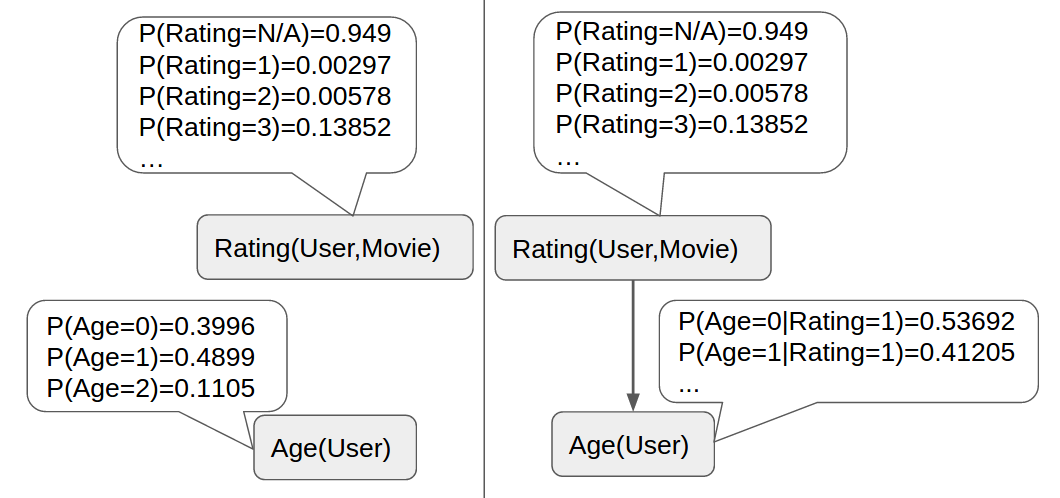
\includegraphics[width=0.48\textwidth] 
	{bnstructIjcai}
	\caption{Example First-Order Bayesian networks: left = $\BN_{1}$  with graph $\graph_{1}$, right = $\BN_{1}^+$ with graph $\graph_{1}^+$. %The type of population variables is shown as in a plate model. 
		\label{fig:bn}}
\end{figure}


\begin{table}[tb]
\caption{The IMDb database frequency of a joint assignment to first-order random variables, compared to the BN probabilities computed using the network parameters of Figure~\ref{fig:bn}.}
\begin{center}
\resizebox{0.5\textwidth}{!}{
\begin{tabular}{|r|r|r|}
\hline
$\set{\Xvariable}=\set{\xvalue}$ & \begin{tabular}{l}$\it{Age(User)=0}$\end{tabular} & \begin{tabular}{l}$\it{Age(User)=0},$\\ $\it{Rating(User,Movie)=1}$\end{tabular}  \\\hline
$\Count{\set{\Xvariable} = \set{\xvalue}}{\dstructure}$ & 376 & 2,524 \\\hline
$\psize{\set{\Xvariable} = \set{\xvalue}}{\dstructure}$ & 941 & 1,582,762  \\\hline 
$\dprob{\dstructure}{\set{\Xvariable} = \set{\xvalue}} $ & $376/941 \approx 0.3996$ & $2,524/1,582,762 \approx 0.0016$ \\\hline
$\bprob{P}{\BN_1}{\set{\node} = \set{\xvalue}}$ & 0.3996 & $0.00297 \cdot 0.3996 \approx 0.0012$ \\\hline
$\bprob{P}{\BN_{1}^+}{\set{\node} = \set{\xvalue}}$ & 0.3996 & $0.00297 \cdot 0.53692 \approx 0.0016$ \\\hline
\end{tabular}
}
\end{center}
\label{table:frequency}
\end{table}%

Figure~\ref{fig:bn} shows an example of two small FOBs. The rating value is n/a (for ``not applicable'') if and only if the user has not rated the movie (cf.~\cite{Russell2010}). {\em Throughout the paper, conditional probability estimates are computed from the IMDb database described below.} Table~\ref{table:frequency} illustrates database frequencies using the IMDb dataset. 
%In the first row, t
The number of users is 941, of which 376 are at age level 0, so the frequency of age 0 users is 376/941. The number of user-movie pairs is 1,582,762 of which 2,524 have the user at age level 0 and a  rating of 1. Marginal and joint BN probabilities are computed using Equation~\eqref{eq:bn}. %On the random selection semantics, a BN probability of $p$ can be read as  ``if we randomly select a user and a movie, the probability is $p$ that the user has age level 1 and rates the movie 1''.  
The expanded BN $\BN_{1}^+$ matches the database distribution perfectly but at the cost of more parameters. 
%For iid data, there are well-explored criteria for making this trade-off. 
%The next section describes how i.i.d criteria for making this trade-off can be upgraded. %to relational data.

%\begin{align*}
%\dprob{\dstructure}{\it{Age(User)} = 0,\it{Rating(User,Movie)} = 1} \\ = 2,524/1,582,762 \approx 0.0016.
%\end{align*}

%$$\dprob{\dstructure}{\it{Age(User)} = 0,\it{Rating(User,Movie)} = 1} = 2,524/1,582,762.$$




%\begin{table}[t]
%\caption{Probabilities for the joint assignment $\it{Age(User)} = 0,\it{Rating(User,Movie)} = 1$ given by the BNs of Figure~\ref{fig:bn}.}
%\begin{center}
%\resizebox{0.48\textwidth}{!}{
%\begin{tabular}{|c|c|c|}
%\hline
%BN & $P_{\BN}$ & \#parameters \\\hline
%$\BN_{1}$  & 0.00297 \cdot 0.3996 \approx 0.0012 & 5+2 = 7 \\\hline
%$\BN_{1}^+$ & 0.00297 \cdot 0.53692 \approx \bf{0.0016} & $5 + 6\times 2 = 17$\\\hline
%\end{tabular}
%}
%\end{center}
%\label{table:bn-frequencies}
%\end{table}%

%Table~\ref{table:bn-frequencies} provides the Figure~\ref{fig:bn} BN probabilities %$\bprob{P}{\BN}{\it{Age(User)=0,Rating(User,Movie)=1}}$ %
%for the same event.
%On the random selection semantics, a BN probability of $p$ can be read as  ``if we randomly select a user and a movie, the probability is $p$ that the user has age level 1 and rates the movie 1''. 



%With the data conditional probabilities, the expanded $\BN_{1}^+$ structure matches the database frequencies better than the disjoint structure $\BN_{1}$, at the cost of multiplying the number of effective parameters. For iid data, there are well-explored criteria for making this trade-off. The next section describes how these criteria can be upgraded to relational data.

%The BN $\BN_{1}$ of Figure~\ref{fig:bn}(left) contains 6+3=9 parameters for five rating levels. The result of Equation~\ref{eq:bn} is 

%\begin{align*}
%\bprob{P}{\BN_1}{\it{Age(User)} = 0,\it{Rating(User,Movie)} = 1}\\ = 0.00297 \cdot 0.3996 \approx 0.0012.
%\end{align*}

%The BN $\BN_{2}$ of Figure~\ref{fig:bn}(right) contains 6+3x6=24 parameters. The result of Equation~\ref{eq:bn} is 

%\begin{align*}
%\bprob{P}{\BN_2}{\it{Age(User)} = 0,\it{Rating(User,Movie)} = 1}\\ = 0.00297 \cdot 0.53692 \approx 0.0016.
%\end{align*}



\section{Multi-Relational Model Comparison} 

%We review model scores for i.i.d. data then discuss upgrading them for multi-relational data.
%We define the relational  model comparison scores that we study in this paper. We begin with general model selection concepts. 
%The model scores we consider have as components a likelihood function and a complexity penalty term. We consider relational likelihood functions, then how to expand them with terms that penalize model complexity. 
%
%\subsection{Model Scores for i.i.d. Data} 
%
%We adapt previously established notation and concepts  for Bayesian network structure scores. 
An i.i.d. score %$\Score{S}{G}{\dset}$% 
measures how well a DAG $\graph$ fits an i.i.d. dataset $\dset$~\cite{Chickering2002}. %,bouckaert95:_bayes}.  
A BN score defines a function $\Score{S}{\graph}{\Fbcount{\graph}{ijk}{\dset}}$ that depends on the graph structure 
 and the \defterm{sufficient statistics} $\Fbcount{\graph}{ijk}{\dset}$. For Bayesian networks, the sufficient statistics are the observed instantiation counts of the possible child-parent configurations. %~\cite{Heckerman1998}. 
Let $\node_{i} = \xvalue_{ik},\Parents{i}{\graph}=\pavalue{ij}{\graph}$ be the assignment that sets node $i$ to its $k$-th value, and its parents to their $j$-th possible configuration. Then $\Fcount{\graph}{ijk}{\dset} \equiv \Count{\node_{i} = \xvalue_{ik},\Parents{i}{\graph}=\pavalue{ij}{\graph}}{\dset}$ is the number of data points that satisfy the $\it{ijk}$ assignment. A standard BN score is {\em decomposable}, that is, the score  can be written as a sum of \defterm{local scores} $S_{i}$, each of which is a function only of one node $\node_{i}$ and its parents:

\begin{equation} \label{eq:decomposable}
\Score{S}{\graph}{\Fbcount{\graph}{ijk}{\dset}} := \sum_{i} \score{S}{i}{G}{\Fbcount{\graph}{ijk}{\dset}}.
\end{equation}
 

We use the following notation for {\em relational} sufficient statistics.

\begin{itemize}
\item $\Fcount{G}{ijk}{\dstructure} \equiv \Count{\node_{i} = \xvalue_{ik},\Parents{i}{G}=\pavalue{ij}{G}}{\dstructure}$ is the number of groundings that satisfy the $ijk$ assignment.
\item $\Fcount{G}{ij}{\dstructure} \equiv \sum_{k} \Fcount{G}{ijk}{\dstructure}$ is the number of groundings that satisfy the $j$-th parent assignment.
\item $\Fcount{G}{i}{\dstructure} \equiv \sum_{j}\sum_{k} \Fcount{G}{ijk}{\dstructure}$ is the number of possible groundings for node $i$.
\end{itemize}

Since the quantity $\Cvar_{i}^{G}$ plays the same role as the sample size in i.i.d. data, we refer to it as the \defterm{local sample size} for node $i$.  
%(Even though the groundings associated with node $i$ do not form an i.i.d. random sample.) 
%
%
%The most straightforward approach is to upgrade an i.i.d. score simply by replacing in Algorithm~\ref{alg:score} the i.i.d. sufficient statistics with the relational sufficient statistics.
%
%The \defterm{count log-likelihood} $\score{\loglikelihood}{i}{\graph}{\dstructure}$ is defined as in Equation~\eqref{eq:iid-loglikelihood}. 

We propose a relational \textbf{gain function} $\Gain{\improve{S}}{G}{G'}{\dstructure}$ that measures how much an alternative structure $G'$ improves a current structure $G$ according to criterion $S$. Our definition focuses on the case where the alternative $\graph'$ adds parents to a node $\node_{i}$ in $\graph$. The case where $\graph'$ removes parents reverses the role of $\graph$ and $\graph'$. This is sufficient for applying standard BN structure search algorithms, which consider adding or deleting a single edge at a time, or distinct phases for adding and deleting edges. %~\cite{Chickering2003}. 
The gain for edge reversals adds the gains for a deletion and addition. Algorithm~\ref{alg:gain} shows pseudo code for the gain function.
Table~\ref{table:gain-examples} gives the normalized gain penalty formulas for upgrading the standard log-likelihood, $\aic$, and $\bic$ scores~\cite{bouckaert95:_bayes}. 
%(Some constant factors are omitted.) 
%\footnote{We omit a constant factor of 2 that does not affect model comparisons.} 
Algorithm~\ref{alg:gain} can be applied with other scores as well (e.g. for $\bdeu$ the normalized gain formula is given in~\cite[Section~3.1.3]{gholami2016upgrading}). We focus on $\aic$ and $\bic$ because they are widely used and have a relatively simple definition.
%Table~\ref{table:gain-examples} shows the gain formulas for standard BN scores.
 
\begin{algorithm}[tb]
%\linesnumbered
\SetKwData{Calls}{Calls}
\SetKwData{Notation}{Notation}
\KwIn{Database $\dstructure$; Bayesian network DAGs $G,G^{+}$ where $\bnparents_{i}^{G} \subseteq \bnparents_{i}^{G^{+}}$ for each node $\Xvariable_{i}$.}
\KwOut{Gain value $\Gain{\improve{\nscore{S}}}{G}{\graph^{+}}{\dset}$}
\Calls local i.i.d. score $\score{S}{i}{G}{\set{\Cvar}_{ijk}}$. (Eq.~\eqref{eq:decomposable})
\begin{algorithmic}[1]
\STATE $\Fpcount{\graph}{ijk}{\dstructure} := \Fbcount{\graph}{ijk}{\dstructure} \times \frac{\Fcount{G^{+}}{i}{\dstructure}}{\Fcount{G}{i}{\dstructure}}$ \label{line:rescale}
\COMMENT{rescale sufficient statistics for graph $G$}
	\FORALL{nodes $i$}
\STATE $\gain{\improve{\nscore{S}}}{i}{G}{\dstructure} := [\score{S}{i}{\graph^{+}}{\Fbcount{\graph^{+}}{ijk}{\dstructure}} - \score{S}{i}{\graph}{\Fpcount{\graph}{ijk}{\dstructure}}]/\Fcount{G^{+}}{i}{\dstructure}$ \label{line:normalize}
\COMMENT{gain = [score of $\graph^+$-scaled score of $\graph$]/local sample size}
\ENDFOR	
\RETURN %$\Gain{\improve{\nscore{S}}}{G}{\graph^{+}}{\dstructure} := 
$\sum_{i} \gain{\improve{\nscore{S}}}{i}{G}{\dstructure}$
\end{algorithmic}
\caption{The normalized gain method upgrades  a decomposable i.i.d. BN score $S$ for multi-relational data.}
\label{alg:gain}
\end{algorithm}

\begin{table*}[tb] \centering
\resizebox{0.9\textwidth}{!}{
\begin{tabular}{| c | c |c|c|}
\hline
 Score $S$ & $\score{S}{i}{\graph^{+}}{\Fbcount{\graph^{+}}{ijk}{\dstructure}}$ &$\score{S}{i}{\graph}{\Fpcount{\graph}{ijk}{\dstructure}}$ & $\gain{\improve{\nscore{S}}}{i}{G}{\dstructure}$ \\ \hline
 $\loglikelihood $ &  
% \begin{tabular}{c}
 $\sum_{j} \sum_{k} \Fcount{\graph^{+}}{ijk}{\dstructure} \cdot
 \log_{2} \left(\frac
{\Fcount{\graph^{+}}{ijk}{\dstructure}}{\Fcount{\graph^{+}}{ij}{\dstructure}}\right)$ 
%\end{tabular}
&  
%\begin{tabular}{c}
$\sum_{j} \sum_{k} \Fpcount{\graph}{ijk}{\dstructure} \cdot 
\log_{2} \left(\frac
{\Fpcount{\graph}{ijk}{\dstructure}}{\Fpcount{\graph}{ij}{\dstructure}}\right)$
%\end{tabular}
& \begin{tabular}{l}
$[\score{\loglikelihood}{i}{\graph^{+}}{\Fbcount{\graph^{+}}{ijk}{\dstructure}}-$ \\ $\score{\loglikelihood}{i}{\graph}{\Fpcount{\graph}{ijk}{\dstructure}}]/\Fcount{G^{+}}{i}{\dstructure}$
\end{tabular}
\\\hline
\aic & $\score{\loglikelihood}{i}{\graph^{+}}{\Fbcount{\graph^{+}}{ijk}{\dstructure}}-\numpars{G^{+}}{i}$ & $\score{\loglikelihood}{i}{\graph}{\Fpcount{\graph}{ijk}{\dstructure}}-\numpars{\graph}{i}$  & 
\begin{tabular}{l}
$\gain{\improve{\nscore{\loglikelihood}}}{i}{G}{\dstructure}+$\\$[\numpars{\graph}{i}-\numpars{G^{+}}{i}]/\Fcount{G^{+}}{i}{\dstructure}$
\end{tabular}\\\hline
\bic & \begin{tabular}{l} $\score{\loglikelihood}{i}{\graph^{+}}{\Fbcount{\graph^{+}}{ijk}{\dstructure}}$-
\\$\log_{2}(\Fcount{\graph^{+}}{i}{\dstructure})/2\cdot \numpars{G^{+}}{i}$  
\end{tabular}
&\begin{tabular}{l} $\score{\loglikelihood}{i}{\graph}{\Fpcount{\graph}{ijk}{\dstructure}}$-
\\$\log_{2}(\Fcount{\graph^{+}}{i}{\dstructure})/2\cdot \numpars{G}{i}$  
\end{tabular}
& 
\begin{tabular}{l}
$\gain{\improve{\nscore{\loglikelihood}}}{i}{G}{\dstructure}+$\\
$\frac{\log_{2}(\Fcount{\graph^{+}}{i}{\dstructure})}{2\Fcount{G^{+}}{i}{\dstructure}}
[\numpars{\graph}{i}-\numpars{G^{+}}{i}]$
\end{tabular}\\\hline
%\bdeu & 
% \begin{tabular}{l}
% $\sum\limits_{j=1}^{\numparents{i}{\graph^{+}}}
% [
% \log\left(\Gamma(\frac{N'}{\numparents{i}{\graph^{+}}})/
% \Gamma(\Fcount{\graph^{+}}{ijk}{\dstructure} + \frac{N'}{\numparents{i}{\graph^{+}}})\right) + $\\
%      $\sum\limits_{k=1}^{\numvalues{i}}\log\left(
%      \Gamma(\Fcount{\graph^{+}}{ijk}{\dstructure}+\frac{N'}{\numvalues{i}\numparents{i}{\graph^{+}}})/
%      \Gamma(\frac{N'}{\numvalues{i}\numparents{i}{\graph^{+}}})\right)
%      ]$
% \end{tabular} &
% \begin{tabular}{l}
% $\sum\limits_{j=1}^{\numparents{i}{\graph}}
% [
% \log\left(\Gamma(\frac{N'}{\numparents{i}{\graph}})/
% \Gamma(\Fcount{\graph}{ijk}{\dstructure} + \frac{N'}{\numparents{i}{\graph}})\right) + $\\
%      $\sum\limits_{k=1}^{\numvalues{i}}\log\left(
%      \Gamma(\Fcount{\graph}{ijk}{\dstructure}+\frac{N'}{\numvalues{i}\numparents{i}{\graph}})/
%      \Gamma(\frac{N'}{\numvalues{i}\numparents{i}{\graph}})\right)
%      ]$
% \end{tabular}
% & \begin{tabular}{l}
% $[\score{\bdeu}{i}{\graph^{+}}{\Fbcount{\graph^{+}}{ijk}{\dstructure}}-$ \\ $\score{\bdeu}{i}{\graph}{\Fpcount{\graph}{ijk}{\dstructure}}]/\Fcount{G^{+}}{i}{\dstructure}$
% \end{tabular}
% \\\hline \hline
%Notation & $\numvalues{i} \equiv $ \#values of $\Xvariable_i$ & $\numparents{i}{H} \equiv$ \#parent configurations of $\Xvariable_i$ &$\numpars{H}{i} \equiv (\numvalues{i}-1) \cdot \numparents{i}{H}$\\
 %\hline 
\end{tabular}
}
\caption{The normalized gain for selected standard 
BN scores. $\loglikelihood$ denotes the log-likelihood score. $\numpars{H}{i}$ denotes the number of parameters for node $\node_{i}$ in DAG $H$. Some constant factors are omitted.  %For \bic~ n
Note that $\overline{\Cvar}^{\graph}_{i}(\dstructure) = \Fcount{\graph^{+}}{i}{\dstructure}.$}
\label{table:gain-examples}
\end{table*}




\paragraph{Motivation}  Rescaling sufficient statistics for the current graph $\graph$ (line~\ref{line:rescale}) makes comparable the scores of the current graph and the alternative graph $\graph^{+}$.  Normalization (line~\ref{line:normalize}) makes comparable the gains for different alternative graphs.
%with different numbers of local instances. 
The normalization measures the gain per local instance.


% We discuss the motivation for our gain function. %line by line.
% \\
% {\em Normalizing sufficient statistics} (Line~\ref{line:rescale}).   The term $\frac{\Fcount{G^{+}}{i}{\dstructure}}{\Fcount{G}{i}{\dstructure}}$ in Line~\ref{line:rescale} rescales the instantiation counts for the smaller structure $\graph$, by multiplying the product of the domain sizes of the population variables that are added to the parent set of node $\node_{i}$ by the new parents from $\graph^{+}$. After normalizing, the local sample sizes are the same for both graphs (i.e., $\overline{\Cvar}_i^{\graph}=\Cvar_i^{\graph^{+}}$).
% \\
% {\em Log-likelihood gain} (Line~\ref{line:ll-gain}).    The log-likelihood gain is computed using the normalized instantiation counts for the smaller structure. If we used the unscaled relational counts, the likelihood score $\score{\loglikelihood}{i}{\graph}{\Fbcount{\graph}{ijk}{\dstructure}}$ would induce an exponential bias against edges that add population variables, which leads to a non-consistent score.
%because if such an edge is required to represent the data generating distribution, it  will not be added even in the sample size limit. 
%
Table~\ref{table:likelihood-example} illustrates the importance of re-scaling counts. The $\score{\loglikelihood}{i}{\cdot}{\Fbcount{\cdot}{ijk}{\cdot}}$ column shows the likelihood score with instantiation counts. This term is an order of magnitude lower for the expanded BN structure $G_{1}^+$ (-2266 vs. -497),  simply because the expanded structure increases the local sample size by the number of Movies. 
% Therefore the count likelihood score is not consistent because it fails to select structures that increase the local sample size by connecting different populations.

% Dividing by the local sample sizes normalizes the likelihood score for different graph structures to the same range. 


\begin{table*}[tb]\centering
\resizebox{0.9\textwidth}{!}{
\begin{tabular}{|l|r|l|r|r|r|r|r|}
\hline
Family Configuration & \multicolumn{1}{l|}{$n_{ijk}$} & $n_{ij}$ & \multicolumn{1}{l|}{$n_{i}$} & \multicolumn{1}{l|}{$n_{ijk}/n_i$} & \multicolumn{1}{l|}{\emph{CP}} & \multicolumn{1}{l|}{$\score{\loglikelihood}{i}{\cdot}{\Fbcount{\cdot}{ijk}{\dstructure}}$} & \multicolumn{1}{l|}{$\frac{\score{\loglikelihood}{i}{\cdot}{\Fbcount{\cdot}{ijk}{\dstructure}}}{\Fcount{G^{+}}{i}{\dstructure}}
$} \\ \hline
\begin{tabular}{l}Age(User)=0\end{tabular} & 376 & --- & 941 & 0.3996 & 0.3996 & -497.6217 & -0.5288 \\ \hline
\begin{tabular}{l}Age(User)=0, \\Rating(User,Movie)=1\end{tabular} & 2524 & \multicolumn{1}{r|}{4703} & 1582762 & 0.0016 & 0.5367 & -2266.2224 & -0.0014 \\ \hline
\end{tabular}
}
\caption{For the node $\it{Age(User)}$, and the IMDb dataset, the contribution of one family configuration to the unnormalized resp. normalized log-likelihood score. Top: For the $G_{1}$ structure of Figure~\ref{fig:bn}. Bottom: For the expanded structure $G_{1}^+$.
\label{table:likelihood-example}}
\end{table*}

% \emph{Gain Normalization} (Line~\ref{line:gain}). 
% %The gain is computed as , normalized by the sample size for the larger graph. 
% Normalizing the difference between the log-likelihood gain and the complexity loss avoids a bias against edges that add population variables with large domains. 
%For example, an alternative structure $H^{+}$ may add an edge $\it{Friend(User,User1)} \rightarrow
%\it{Age(User)}$ to represent an auto-correlation of a user's age with that of her friends. The local sample size for $H^{+}$ is $|\it{Users}| \times |\it{Users}|$, 
%contains 941 users, the local sample size in $H^{+}$ is $941^{2} = 885,481$ 
%compared to $|\it{Users}| \times |\it{Movies}|$ for the structure $\graph_{1}^{+}$. Without normalization, the gain function would favor the structure $H^{+}$ over $\graph_{1}^{+}$ simply because its counts are on a smaller scale.

\paragraph{Relationship to Normalized Likelihood} In previous work on parameter learning, \cite{Xiang2011,Schulte2011}, the log-likelihood score $\loglikelihood$ was upgraded by the \defterm{normalized log-likelihood score} NLL
$$
  \score{\nscore{\loglikelihood}}{i}{G}{\Fbcount{G}{ijk}{\dstructure}}
  \equiv  \score{\loglikelihood}{i}{\graph}{\Fbcount{G}{ijk}{\dstructure}}/\Fcount{G}{i}{\dstructure},
$$ which converts log-likelihood scores to the same scale, as shown in Table~\ref{table:likelihood-example}. 
%The next observation shows that t
The normalized gain for the log-likelihood score is equivalent to the normalized log-likelihood score differential.

\begin{observation} \label{prop:nll}
The normalized gain equals the difference in normalized log-likelihood. In symbols: 
$$\gain{\improve{\nscore{\loglikelihood}}}{i}{\graph}{\dstructure}=
\score{\nscore{\loglikelihood}}{i}{\graph^{+}}{\Fbcount{\graph^{+}}{ijk}{\dstructure}} - \score{\nscore{\loglikelihood}}{i}{\graph}{\Fbcount{\graph}{ijk}{\dstructure}}.$$
\end{observation}

\emph{Proof.} It suffices to show that $\score{\loglikelihood}{i}{\graph}{\Fpcount{\graph}{ijk}{\dstructure}}/\Fcount{G^{+}}{i}{\dstructure}=\score{\loglikelihood}{i}{\graph}{\Fbcount{\graph}{ijk}{\dstructure}}/\Fcount{G}{i}{\dstructure}$. In the scaled log-likelihood $\score{\loglikelihood}{i}{\graph}{\Fpcount{\graph}{ijk}{\dstructure}}$, the scale factor $\frac{\Fcount{G^{+}}{i}{\dstructure}}{\Fcount{G}{i}{\dstructure}}$ does not affect the conditional probability ratio, and can be moved to the front of the sum. Therefore $$\score{\loglikelihood}{i}{\graph}{\Fpcount{\graph}{ijk}{\dstructure}}=
\frac{\Fcount{G^{+}}{i}{\dstructure}}{\Fcount{G}{i}{\dstructure}}
\score{\loglikelihood}{i}{\graph}{\Fbcount{\graph}{ijk}{\dstructure}}.$$

Many standard BN scores, such as  $\aic$ and $\bic$, are {\bf likelihood scores} that combine the maximum likelihood of the data under the model with a {\em penalty} term $\spenalty{S}{i}{G}{\Fbcount{G}{ijk}{\dset}}$ that is a function of the number of parameters and the sample size \cite{bouckaert95:_bayes}. Observation~\ref{prop:nll} implies that the normalized gain for likelihood scores is equivalent to adding a normalized penalty term to the normalized likelihood. Whereas the normalized likelihood gain can be represented as the difference of two fixed single-model scores, this is no longer true for likelihood scores with penalty terms, because the scaling factor $\Fcount{G^{+}}{i}{\dstructure}$ is applied to the current graph but depends on the alternative graph. 
%Since we depart from the traditional single-model score framework, 
Our evaluation compare the gain function concept  with single-model scores as baselines.

\paragraph{Comparison With Single-Model Likelihood Scores.} 
%We consider upgrading likelihood scores. % such as $\aic$ and $\bic$. 
The simplest approach to upgrading an i.i.d. score is to use it with relational instance counts (i.e., $\score{S}{i}{\graph}{\Fbcount{\graph}{ijk}{\dstructure}}$). However, this approach has the serious drawback that when a new edge increases the local sample size by connecting different populations, the likelihood  decreases while the model complexity increases (see Table~\ref{table:likelihood-example}). Therefore an instance count likelihood score is not consistent, because it fails to add  edges that introduce new population variables, no matter how large the sample size (see \cite{Schulte2016a} for empirical confirmation). Our comparison therefore uses likelihood scores that extend the {\em normalized} log-likelihood score $\nscore{\loglikelihood}$ %established in previous work 
with a penalty term. The count method simply adds the penalty term; the normalized method divides it by the local sample size, which %by Observation~\ref{prop:nll} 
is equivalent to normalizing the instance count score (i.e. $\score{S}{i}{\graph}{\Fbcount{\graph}{ijk}{\dstructure}}/\Fcount{G}{i}{\dstructure}$).


% \begin{equation}
% \scriptsize
% \label{eq:diff}
%   \gain{\improve{\loglikelihood}}{i}{G}{\dstructure}/\Fcount{G^{+}}{i}{\dstructure} = \score{\nscore{\loglikelihood}}{i}{\graph^{+}}{\Fbcount{\graph^{+}}{ijk}{\dstructure}} - \score{\nscore{\loglikelihood}}{i}{\graph}{\Fbcount{\graph}{ijk}{\dstructure}}
% \end{equation}

% our gain function can be seen as extending the normalized log-likelihood score %established in previous work 
% with a normalized penalty term. 
% Building on the previous work, our single-model score upgrade methods add a penalty term to the normalized log-likelihood score.
%$\score{\nscore{\loglikelihood}}{i}{G}{\Fbcount{G}{ijk}{\dstructure}}$: 
% The count method simply applies the i.i.d. score with relational sufficient statistics; the normalized method divides the count score by the local sample size. 

\begin{description}
\item[Count]
{\small $\score{\nscore{\loglikelihood}}{i}{G}{\Fbcount{G}{ijk}{\dstructure}}- \spenalty{S}{i}{G}{\Fbcount{G}{ijk}{\dset}}$}
\item[Normalized] \small $\score{\nscore{\loglikelihood}}{i}{G}{\Fbcount{G}{ijk}{\dstructure}}-\spenalty{S}{i}{G}{\Fbcount{G}{ijk}{\dstructure}}/\Fcount{G}{i}{\dstructure}$
\end{description}

%The baseline methods  define relational scores by normalizing the likelihood term and/or the penalty term. This upgrade scheme defines 4 different relational versions of a model selection score; see Table~\ref{table:compare-design}. Normalizing the penalty term but not the likelihood term is clearly inadequate.

Table~\ref{table:comparison-scores} gives the corresponding formulas for the $\aic$ and $\bic$  penalty terms. 
%For such likelihood-based scores, our single-model score upgrade methods add a penalty term to the normalized log-likelihood. 
Table~\ref{table:compute-scores} shows example values for the scores and gains. 

\begin{table}[tb]
% \resizebox{0.5\textwidth}{!}{
\begin{tabular}{| p{2.7cm} | c | c |}
	\hline Criterion & $\aic_{i}$ & $\bic_{i}$  \\
	\hline
%  Normalized Gain & $\frac{(\numpars{G^{+}}{i} - \numpars{G}{i})}{\Fcount{\graph^{+}}{i}{\dstructure}}$
% & $(\numpars{G^{+}}{i} - \numpars{G}{i}) \cdot \frac{\log_{2}(\Fcount{\graph^{+}}{i}{\dstructure})}{2 \Fcount{\graph^{+}}{i}{\dstructure}}$ \\
% \hline

Count Score 
& $ \numpars{G}{i}$
&$ \numpars{G}{i} \cdot \frac{1}{2}\log_2(\Fcount{G}{i}{\dstructure}) $

\\\hline
 Normalized Score  & 
$ \frac{\numpars{G}{i}}{\Fcount{G}{i}{\dstructure}}$ &
$  \numpars{G}{i} \cdot \frac{\log_2(\Fcount{G}{i}{\dstructure}}{2 \Fcount{G}{i}{\dstructure}}$ \\\hline
\end{tabular}
%} % end box
\caption{Relational Penalty Terms for the $\aic$ and $\bic$ scores. 
%The gain penalty is $\gain{\improve{f^{S}}}{i}{G}{\dstructure}/\Fcount{G}{i}{\dstructure}$ (Algorithm~\ref{alg:gain} Line~\ref{line:penalty-gain}). 
The evaluated scores add the penalty term to the normalized log-likelihood $\nscore{\loglikelihood}$.}
%defines the model selection criteria used in our experiments.} 
\label{table:comparison-scores}
\end{table}


\begin{table*}[tb]\centering
\resizebox{0.9\textwidth}{!}{
\begin{tabular}{|l|c|c|c|c|c|c|c|c|c|}
\hline
 \multicolumn{1}{|l|}{} & \multicolumn{1}{l|}{} & \multicolumn{1}{l|}{} & \multicolumn{1}{c|}{} & \multicolumn{3}{c|}{AIC} & \multicolumn{3}{c|}{BIC}  \\ \hline
 & \multicolumn{1}{l|}{\#groundings} & \multicolumn{1}{l|}{\#parameters} & \multicolumn{1}{l|}{$\nscore{\loglikelihood}$} &  \multicolumn{1}{l|}{count} & \multicolumn{1}{l|}{normalized gain} & normalized & \multicolumn{1}{l|}{count} & \multicolumn{1}{l|}{normalized gain} & normalized \\ \hline
    $G_{1}$ & 941 & 2 & -1.384 &  -3.38 & ---  & -1.3865  & -11.26 & --- & -1.3948 \\%\hline
    $G_{1}^{+}$ & 1582762 & 12 & -1.177  & -13.18 & --- & -1.1775  & -124.74 & --- & -1.1776 \\ \hline
    GAIN &  & 10 & 0.207  & -9.79 & 0.20684 & 0.2090  & -113.48 & 0.20678 & 0.2173  \\\hline
\end{tabular}
}
\caption{Example values for the scores and gain functions defined in this section, for the IMDb dataset and the structures of Figure~\ref{fig:bn}. Note that count gain $<$ normalized gain $<$ normalized score gain. E.g., for $\aic$ gains  $ -9.79 < 0.020684  < 0.2090$.
\label{table:compute-scores}}
\end{table*}

%In general, the gain function values are ordered as count gain $<$ normalized gain $<$ normalized score gain. 
%This is appropriate because previous work used  the normalized log-likelihood score  an objective function for {\em parameter} learning and did not consider structure learning. 
% \begin{equation} \label{eq:normalized-loglikelihood}
%   \score{\nscore{\loglikelihood}}{i}{G}{\Fbcount{G}{ijk}{\dstructure}}
%   \equiv \frac{1}{\Fcount{G}{i}{\dstructure}} \score{\loglikelihood}{i}{\graph}{\Fbcount{G}{ijk}{\dstructure}}
% \end{equation}


% The gain function is a novel concept distinct from a
% single-model score.  As we discussed below, previous work has shown that non-rescaled sufficient statistics lead to an inadequate log-likelihood score. 
 

\section{Theoretical Consistency Analysis}

%These observations lead to a difference in theoretical performance guarantees: whereas upgrading an i.i.d score with the normalized gain function preserves the consistency of the i.i.d. score, upgrading the single model score functions does not. 
% A large sample analysis considers a sequence of samples from the true data generating distribution that grow without bound. A model selection method is consistent if the sequence of models that it selects converges to one that is correct for the data generating distribution. 
We formalize consistency for relational data following previous work~\cite{Sakai2013,Xiang2011}. %,Shalizi2013}.
%,  
%we formalize these concepts as follows. 
%In the limit each population size $\individuals_{i}$ goes to infinity, 
%$\psize{\individuals_{i}}{\dstructure_{j}} \rightarrow \infty$,
%which like \citeauthor{Sakai2013} we 
%abbreviate 
%denote as 
The notation $\set{\samplesize}(\dstructure) \rightarrow \infty$ from 
denotes that  each population size $\individuals_{i}$ goes to infinity. %\cite{Sakai2013} . 
Similar to \citeauthor{Sakai2013}, we make the identifiability assumption that %\\
\begin{equation}
   \dprob{\dstructure}{\cdot}\rightarrow\dprob{\structure}{\cdot} \equiv p  \mbox{ as } \set{\samplesize}(\dstructure) \rightarrow \infty,
   \label{eq:identifiability}\end{equation}
%
where $\structure$ represents a complete relational structure (network) from which samples are drawn, and $p$ denotes the generative distribution associated with $\structure$. This assumption holds under various sampling schemes such as subgraph sampling \cite{Frank1978}.\footnote{Assumptions for consistent parameter learning in PRMs (but not SRMs) are discussed in several papers ~\cite{Xiang2011,Shalizi2013,Sakai2013}.}
%It is well-known that a BN structure $\graph$ can be parametrized to represent a distribution $p$ if and only if $\graph$ is an I-map of $p$, meaning that every conditional dependence in $p$ corresponds to d-separation in $\graph$ \cite{Pearl1988}. A model score is therefore (globally) consistent if, given an arbitrarily large sample from a $p$, the score-optimal structures are I-maps of $p$. 
%for brevity.
%and compatibility with \cite{Chickering2003} where $p$ is used for the data generating distribution.
%
%Let $\dstructure_{1},\ldots,\dstructure_{j},\ldots$ be a sequence of databases sampled from structure $\structure$. The data sequence \defterm{converges} if, as $j \rightarrow \infty$,
%
%\begin{enumerate}
%\item $\dprob{\dstructure_{j}}{\cdot}\rightarrow\dprob{\structure}{\cdot} \equiv p$, and [state this as assumption]
%\item $\psize{\individuals_{i}}{\dstructure_{j}} \rightarrow \infty$ for each population $\individuals_{i}$. We abbreviate this as $\set{\samplesize} \rightarrow \infty$.\footnote{Arbitrarily large samples can be generated either by sampling with replacement, or by sampling from infinite populations. The definition of the relational frequency $\dprob{\structure}{\cdot}$ with infinite populations is worked out by \cite{Halpern1990}. The basic idea is to assume that $\structure$ defines a probability measure over tuples of individuals, so the probability $\dprob{\structure}{\set{\Xvariable} = \set{\xvalue}}$ of an assignment is the mass of the set of groundings that satisfy the assignment.}
%\end{enumerate}
%
%A BN structure learning method method is consistent if in the large sample limit, the graph it selects is an I-map for $p$. This means that there is a Bayesian network $G =  (G,\set{\Parentsrameter})$ such that $\dprob{G}{\cdot} = p(\cdot)$.
Chickering and Meek %\citeyear{Chickering2002} 
introduced the concept of  \defterm{local consistency}, which we adapt for %score 
gain functions.
%as follows.

\begin{definition}
% Let $\dstructure$ be a database with sample size vector $\set{\samplesize}$, and 
 Let $p$ be the data generating distribution. A gain function is \defterm{locally consistent} if the following hold % in the sample size limit 
 as $\set{\samplesize}(\dstructure) \rightarrow \infty$, for any graph $\graph$ and expansion $G_{+}$ that adds a single edge $\node_{+} \rightarrow \node_{i}$ to $\graph$:

%\begin{enumerate}
%\item If $\node_{+}$ is not independent of $\node_{i}$ given  $\Parents{i}{G}$ in $\dprob{\structure}{\cdot}$, then $\Gain{\Delta}{G}{G_{+}}{\dstructure_{m}} > 0$.
%\item If $\node_{+}$ is independent of $\node_{i}$ given  $\Parents{i}{G}$ in $\dprob{\structure}{\cdot}$, then $\Gain{\Delta}{G}{G_{+}}{\dstructure_{m}} < 0$.
%\end{enumerate}


\begin{enumerate}
\small
\item If $\node_{+}$ is not independent of $\node_{i}$ given  $\Parents{i}{G}$ in $p$, then $\Gain{\Delta}{G}{G_{+}}{\dstructure} > 0$. \label{clause:consistency}
\item If $\node_{+}$ is independent of $\node_{i}$ given  $\Parents{i}{G}$ in $p$, then $\Gain{\Delta}{G}{G_{+}}{\dstructure} < 0$. \label{clause:optimality}
\end{enumerate}

\end{definition}
%


An upgrade method \defterm{preserves local consistency} if local consistency for an i.i.d. gain function entails local consistency for its upgrade. In the sample size limit, clause~\ref{clause:consistency} entails that 
the gain of a DAG model is (1) positive for any edge that is necessary for eliminating an independence constraint that does not hold in the generative distribution, and (2) is negative for any edge that is unnecessary. Together, these clauses ensure consistency---necessary edges are learned---and optimality---only necessary edges are learned~\cite{Chickering2002}.
%, since it guarantees that the selected structure eventually eliminates all independence constraints that do not hold in the generative distribution. % requires that edges that represent valid dependencies receive a positive gain.  The second clause requires that redundant edges that do no represent a valid dependency receive a negative gain. The first clause is equivalent to global consistency~\cite{Chickering2002}. 
%\footnote{Local implies global: If a structure $\graph$ is not an I-map of the data-generating distribution, it must be missing an edge $\node^{+} \rightarrow \node$ where $\node$  is not independent of $\node^{+}$ given the parents of $\node$ in $\graph$. By Clause 1 of local consistency, such an edge receives a positive gain score. So there is a structure $\graph^{+}$ with a positive gain over $\graph$, and $\graph$ does not optimize the gain function. Global implies local: If a score fails to select a required edge, it fails to select an I-map.}
%Thus any structure $\graph$ that optimizes a locally consistent gain function in the sample size limit is an I-map of the data generating distribution. }
%Clause 2 entails that a locally consistent gain function selects graphs that are optimal in the sense that they do not contain redundant edges. 
% Our main theorem is that the upgrade Algorithm~\ref{alg:gain} preserves local consistency but the single-model scores do not.
\begin{theorem} \label{th:consistency}
The normalized gain upgrade %(Section~\ref{sec:gain})  
preserves local consistency, and therefore consistency. The single-model comparison scores do not preserve local consistency.
\end{theorem}
 
Appendix~\ref{sec:proof} gives the local consistency proof for the normalized gain upgrade method. We provide the intuition rather than a formal proof, for why the single-model scores are not locally consistent. The count score fails Clause~\ref{clause:consistency} because neither the NLL nor the parameter count increase with sample size.  E.g., if $G_{1}^{+}$ is correct, its parameter count is 12, whereas the NLL is -1.177 (in Table~\ref{table:compute-scores}). The penalty term will remain much bigger than the NLL even at large samples from $G_{1}^{+}$.

The normalized score fails Clause~\ref{clause:optimality} because the number of parameters are divided by the local sample sizes. Adding a redundant edge can increase the NLL {\em and} decrease the normalized parameter count. For example, the  parameter count 12 for $G_{1}^{+}$ is divided by 1,582,762, whereas the parameter count 2 for $G_{1}$ is divided by only 941 (Table~\ref{table:compute-scores}). So even if $G_{1}$ is optimal, $G_{1}^{+}$ will receive a higher normalized score even at large samples drawn from $G_{1}$.
This analysis predicts that the count score selects overly sparse structures, and the normalized score overly dense structures.
%, and the normalized gain strikes a desirable balance. 


\section{Empirical Evaluation} 


%We describe the d system and the datasets we used.
%Code was written in Java, JRE 1.7.0.  and executed with 8GB of RAM and a single Intel Core 2 QUAD Processor Q6700 with a clock speed of 2.66GHz (no hyper-threading). The operating system was Linux Centos 2.6.32. 
%The MySQL Server version 5.5.34 was run with 8GB of RAM and a single core processor of 2.2GHz. 
\textbf{Code and Datasets} Our code is available on-line.\footnote{ \url{github.com/sfu-cl-lab/FactorBase_Consistent}}
We used six benchmark real-world databases from the CTU Prague Relational Learning Repository, described in ~\cite{Motl2015a} (also available\footnote{\url{www.cs.sfu.ca/~oschulte/jbn/}} in text format). %For detailed descriptions, please see~\cite{Qian2014a}. %~\cite{Schulte2012,Qian2014a}. 
Table~\ref{table:datasetsize} summarizes basic information about the benchmark datasets.   IMDb is the largest dataset in terms of number of total table tuples (more than 1.3M tuples) and schema complexity. %attributes.
It combines the MovieLens database %\footnote{www.grouplens.org, 1M version} 
with the Internet Movie Database (IMDb).
%following \cite{Peralta2007}.
\footnote{\url{grouplens.org}, 1M version; 
\url{IMDb.com}, July 2013}


% \begin{figure*}[tb]
% 	\centering
% 	\includegraphics[width=0.7\textwidth] 
% 	{abicPlot.png}
% 	\caption{KLD with database distribution and Number of Parameters for different relational score upgrade methods. The number of parameters is shown on log-scale. Top: $\aic$ upgrades. Bottom: $\bic$ upgrades.
% 		\label{fig:scores}}
% \end{figure*}


\begin{table}[tb] \centering
%\scalebox{0.7in}{
\resizebox{0.4\textwidth}{!}{
\begin{tabular}[c]
{|l|c|c|r|c|}\hline
 \textbf{Dataset} & \textbf{\begin{tabular}[l] {ll} \#Relationship \\Tables/ Total \end {tabular}} & \textbf{\#Tuples} & \textbf{\#Attributes}  \\\hline
% \textbf{Dataset} & \textbf{Relationships} & \textbf{\begin{tabular}[l] {ll} Self \\Relationships \end {tabular}} &
% \textbf{\begin{tabular}[l] {ll} Same Type\\ Relationships \end {tabular}}& \textbf{\#Tuples} & \textbf{\begin{tabular}[l] {ll} \#Attribute  \\Columns \end{tabular}}  \\\hline
 University&2 & 171 & 12\\\hline
    Movielens &1 / 3   & 1,010,051 & 7\\\hline
%    Movielens(0.1M) &1 & N & N &  83,402 & 7\\\hline
    Mutagenesis & 2 / 4 & 14,540 & 11\\\hline
    Financial &3 / 7   &  225,932& 15\\\hline
   Hepatitis &3 / 7  &12,927  & 19\\\hline
   IMDb &3 / 7  &1,354,134  & 17\\\hline 
\end{tabular}
}
 % end scalebox
\caption{Datasets characteristics. \#Tuples = total number of tuples over all tables in the dataset. The datasets contain multiple relationships and populations of different types.
  \label{table:datasetsize}}
\end{table}


\noindent\textbf{Model Search Algorithm}
We used the previous learn-and-join method (LAJ) for relational BN model search 
%in relational databases 
\cite{Schulte2012}, with the  implementation provided by its creators. The LAJ method conducts a search through the lattice of relational paths, similar to the iterative deepening strategy of \cite{friedman1999learning}. At each lattice point, an i.i.d. Bayesian network learner is applied, and learned edges are propagated from shorter paths to longer paths. We reconfigured the LAJ algorithm by changing the $\tt{score}$ class for each of the 6 upgraded criteria. 
%for each of the 2 gains,  and each of the 4 scores defined in Table~\ref{table:comparison-scores}.


% \begin{figure}[t]
% 	\centering
% 	\includegraphics[width=0.5\textwidth] 
% 	{kld_count.png}
% 	\caption{KLD for the BIC count-count score \label{fig:kld_count}}
% \end{figure}

\begin{figure}[tbhp]
%gets messed up if replace by [tb]
	\centering
	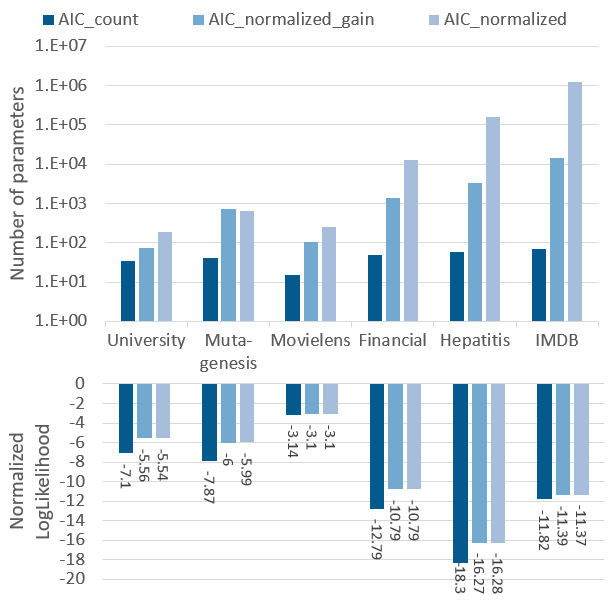
\includegraphics[width=0.5\textwidth,height=240px] 
	{aicPlot.png}
	\centering
	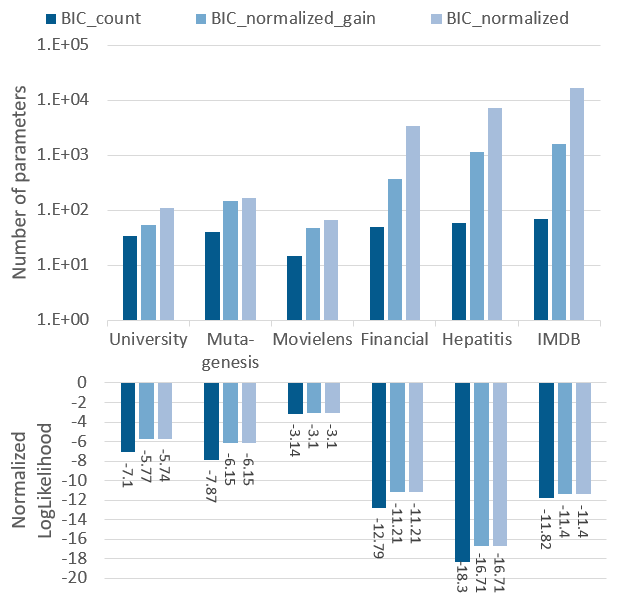
\includegraphics[width=0.5\textwidth,height=240px] 
	{bicPlot.png}
	\caption{Log-likelihood and Number of Parameters for different relational score upgrade methods. 
	%The number of parameters is shown on log-scale. 
	Top: $\aic$ upgrades. Bottom: $\bic$ upgrades.
		\label{fig:scores}}
\end{figure}


\paragraph{Results} 



For each learned graph $G$, we use maximum likelihood estimates to obtain a Bayesian network $\BN$ to be evaluated. We report the normalized log-likelihood (NLL) of the input data and the number of parameters for each learned graph. The likelihood is the natural evaluation measure for generative learning \cite{VanHaaren2016}.
% for both i.i.d.  \cite{Koller2009,Murphy2012} and relational data \cite{VanHaaren2016}.
%
Figure~\ref{fig:scores} shows the metrics for the different upgrade methods. 

\emph{Count Score.}
On each dataset, the count score introduces {\em no} edges, therefore the smallest number of parameters (for instance 69 on IMDb for AIC count vs. 14,450 for normalized gain). Its NLL metric is substantially worse than the gain NLL on 4/6 databases (e.g. on Financial -12.79 for AIC count vs. -10.79 for the normalized gain). The relatively small absolute difference in NLL on MovieLens and IMDb is due to weak correlations and large local sample sizes. 
%For instance on IMDb, the average sample size over nodes for the BIC gain structure is $8\times 10^{11}$. 
{\em We conclude that the count score structures are overly sparse.}

\emph{Normalized Score.} 
On each dataset, the normalized score produces the largest number of parameters (for instance 1,199,853 on IMDb for AIC count vs. 14,450 for normalized gain). The normalized gain function achieves almost the same NLL with many fewer parameters. {\em We conclude that the count score structures are overly dense.}


\begin{figure}[tb]
	\centering
	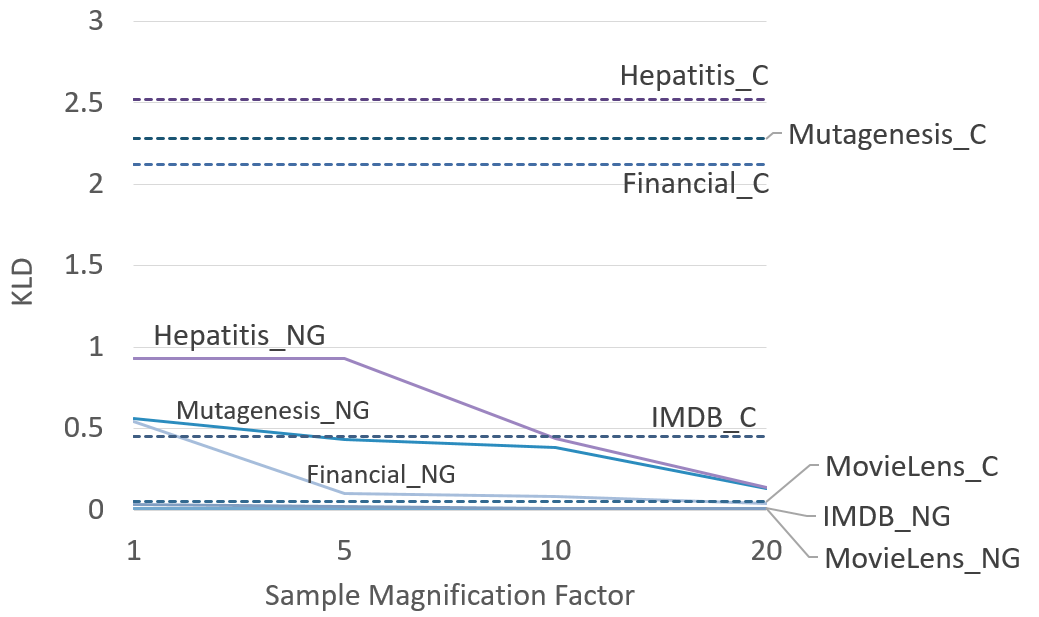
\includegraphics[width=0.44\textwidth] 
	{kld.PNG}
	\caption{BN learning curves for the BIC normalized gain criterion (labelled as "dataset"\_NG) and the count score (labelled as "dataset"\_C). The normalized gain BNs converge to the database distribution (KLD = 0). The BIC count score (\_C) selects the empty graph on all data sets, so its KLD remains constant. \label{fig:kld_ng}}
\end{figure}

\emph{Consistency.} The BIC score is consistent for i.i.d. data~\cite{Chickering2002}, so Theorem~\ref{th:consistency} entails that the BIC normalized gain is also consistent for relational data. Figure~\ref{fig:kld_ng} empirically verifies the consistency of the normalized gain criterion, by showing the convergence to the database distribution on our benchmark databases, meaning that the standard Kulback-Leibler divergence (KLD) metric goes to 0. %~\cite{Campos2006}.  
  Similar to previous experiments~\cite{Getoor2001,Schulte2014}, we duplicate entities by a magnification factor of $m = 1, 5, 10, 20$, which multiplies  local sample sizes by $m$. (We leave out the small  University dataset where convergence requires a higher magnification factor.) The BIC count score adds no edges even with larger sample sizes, so it fails to be consistent. The BIC normalized score outputs a denser graph with KLD equivalent to the normalized gain score (Figure~\ref{fig:scores}). So it is consistent but not locally consistent because it selects redundant edges.  %This is a sampling-with-replacement variation of the design in . 


\section{Conclusion and Future Work} Generalizing i.i.d. model scores designed for i.i.d. data is an important fundamental topic for relational learning. The normalized gain, which measures the difference in data fit between two BN structures, is a novel scalable method for generalizing a Bayesian network score. For complete data, it can be computed in closed form given the BN sufficient statistics. Normalized gain functions preserve the convergence guarantees of i.i.d. scores, and show good empirical performance: they select structures that succinctly represent the data correlations, compared with baseline single-model scores.
%two key properties of i.i.d. BN scores: consistency and balance, meaning that the model's data likelihood  and the model's complexity are measured on the same scale. A surprising negative result is that these properties cannot be achieved with log-linear likelihood scores that are a function of a single model only. Empirical results demonstrate a special strength of the normalized gain upgrade method:  finding arcs whose source node contains population variables that are not included in the child node (e.g. $\it{Rating(User,Movie)} \rightarrow \it{age(User)}$). 

A promising avenue for future work is to apply our approach to other statistical-relational models, such as Markov Logic Networks.
%~\cite{Kimmig2014}. It should be possible to develop a gain function for the log-linear likelihood of Markov Logic Networks.
%As for other Bayesian network relational models, Kersting and deRaedt suggest translating aggregation-based likelihoods into (the equivalent of) a FOB by adding complex aggregate terms as nodes~\cite{Kersting2007}. %Recent results on representing combining rules in a logistic regression model suggest that similar complex terms can be defined  for combining rules~\cite{Buchman2015}. 
%Since our theoretical analysis makes no assumptions about the internal structure of the first-order random variables, it would also apply to Bayesian networks that include complex terms for representing aggregation or combining rules. 
Implementing a BN structure learning system for functors that represent complex terms  would allow us to apply the normalized gain score with aggregate functions/combining rules. 
%This has the potential to address both the question of consistency and the issue of cyclicity. 
%Another important way to expand the space of relational patterns beyond what we examined in this paper is to consider first-order terms that contain constants. 

%  The normalized gain is a novel scalable upgrade method that preserves the consistency guarantees of i.i.d. model selection scores, and shows good empirical performance. 

% \section*{Acknowledgments} This research was supported by a Discovery Grant from the Natural Sciences and Engineering Research Council of Canada. We are indebted to Mark Schmidt and Leonid Chindelevitch for helpful suggestions.

\appendix
\section{Local Consistency Proof for the Normalized Gain Upgrade Method (Theorem~\ref{th:consistency})} \label{sec:proof}
%\section{References}\

We show the local consistency of the rescaled gain, which is the normalized gain with rescaled sufficient statistics but without dividing by the local sample size:

\begin{equation}
\label{eq:rescale}
\Gain{\improve{R}}{G}{\graph^{+}}{\dset} \equiv \score{S}{i}{\graph^{+}}{\Fbcount{\graph^{+}}{ijk}{\dstructure}} - \score{S}{i}{\graph}{\Fpcount{\graph}{ijk}{\dstructure}}
\end{equation}


Since the rescaled gain has the same sign as the normalized gain, {\em proving the local consistency of the rescaled gain implies the local consistency of the normalized gain.}
We say that an edge \defterm{adds a population variable} if the parent contains a population variable that is not contained in the child.

Case 1: The additional edge $\node_{+} \rightarrow \node_{i}$ adds no population variables. For such edges, the rescaled counts are the same as the nonscaled counts used in the original i.i.d. score (i.e., $\Fpcount{\graph}{ijk}{\dstructure} = \Fbcount{\graph}{ijk}{\dstructure}$). So the arguments of~\cite{Chickering2002} can be applied to relational data, and the rescaled gain score is locally consistent in this case. 


Case 2: The additional edge $\node_{+} \rightarrow \node_{i}$ adds a population variable. For concreteness, assume that the edge is of the form $g(\Avariable,\Bvariable) \rightarrow f(\Avariable)$, so the added sample size is $\varsize{\Bvariable}{\dstructure}$. Consider a transformed database $\dstructure'$ where $f(\Avariable)$ is replaced by $f'(\Avariable,\Bvariable)$, with an inert second argument: $f'(\aconstant,\bconstant) = f(\aconstant)$. Since in the transformed schema, the additional edge $\node_{+} \rightarrow \node'_{i}$ does not add a population variable, from case 1 we conclude that (i) the rescaled gain is locally consistent when applied to the transformed data $\dstructure'$. We next show that local consistency for $\dstructure'$ data implies local consistency in $\dstructure$ data. The transformation does not change the information content and is equivalent to rescaling counts:

$$\Fbcount{\graph}{ijk}{\dstructure'} = 
\Fbcount{\graph}{ijk}{\dstructure} \times \varsize{\Bvariable}{\dstructure} = \Fpcount{\graph}{ijk}{\dstructure}.$$ 

Since we also have $\Fbcount{\graph_{+}}{ijk}{\dstructure'} = 
\Fbcount{\graph_{+}}{ijk}{\dstructure}$, the transformed and the original data agree on the  rescaled gain:

\begin{equation} \label{eq:equiv-score}
\Gain{\improve{R}}{G}{\graph^{+}}{\dstructure} = \Gain{\improve{R}}{G}{\graph^{+}}{\dstructure'},
\end{equation}

and agree on the conditional probabilities of a child node value given parent node values:
\begin{equation}
\frac
{\Fcount{\graph}{ijk}{\dstructure}}{\Fcount{\graph}{ij}{\dstructure}} = \frac
{\Fcount{\graph}{ijk}{\dstructure'}}{\Fcount{\graph}{ij}{\dstructure'}}.
\end{equation}

Therefore the identifiability condition~\eqref{eq:identifiability} for the original data $\dstructure$ entails that in the sample size limit, the transformed data $\dstructure'$ identify whether node $\node_{i}$ is independent of $\node_{+}$ given its parents in the data generating distribution $p$. So by condition~\eqref{eq:equiv-score}, the rescaled gain is locally consistent for the original data $\dstructure$. 
 Hence in either case, the normalized gain is locally consistent.

\bibliographystyle{named}
\bibliography{master}

\end{document}

$
\aiclocal{G}{i}{\dstructure} \equiv \dlogcount{G}{i}{\dstructure} - \numpars{G}{i}
$	&
$\aicimprove{G}{G'}{i}{\dstructure} \equiv \frac{\dlogcount{G'}{i}{\dstructure}}{\Fcount{G'}{i}{\dstructure}} - 
\frac{\frac{\Fcount{G'}{i}{\dstructure}}{\Fcount{G}{i}{\dstructure}}\dlogcount{G}{i}{\dstructure}}{\Fcount{G'}{i}{\dstructure}} + \frac{\numpars{G'}{i} - \numpars{G}{i}}{\Fcount{G'}{i}{\dstructure}}$

\begin{equation*}
\dlogcount{G}{i}{\dstructure} \equiv \sum_{j} \sum_{k} \ln \left( \frac
{\Fcount{G}{ijk}{\dstructure}}
{\Fcount{G}{ij}{\dstructure}}\right) \cdot \Fcount{G}{ijk}{\dstructure}
\end{equation*}

\begin{equation*}
\aiclocal{G}{i}{\dstructure} \equiv \dlogcount{G}{i}{\dstructure} - \numpars{G}{i}
\end{equation*}

\begin{equation*}
\logimprove{G}{G'}{i}{\dstructure} \equiv \frac
{\Fcount{G'}{i}{\dstructure}}
{\Fcount{G}{i}{\dstructure}}
\dlogcount{G}{i}{\dstructure} - \dlogcount{G'}{i}{\dstructure}
\end{equation*}

\begin{equation*}
\aicimprove{G}{G'}{i}{\dstructure} \equiv \logimprove{G}{G'}{i}{\dstructure} - \numpars{G}{i} + \numpars{G'}{i}
\end{equation*}

\begin{equation*}
\biclocal{G}{i}{\dstructure} \equiv \dlogcount{G}{i}{\dstructure} - log(\numpars{G}{i})
\end{equation*}


\begin{equation*}
\bicimprove{G}{G'}{i}{\dstructure} \equiv \logimprove{G}{G'}{i}{\dstructure} - log(\numpars{G}{i}) + log(\numpars{G'}{i})
\end{equation*}

\begin{table*}[tb]
\caption{The IMDb database frequency of a joint assignment to first-order random variables, compared to the BN marginal and joint probabilities in  the networks of Figure~\ref{fig:bn}.}
\begin{center}
\resizebox{1.0\textwidth}{!}{
\begin{tabular}{|l|r|r|r|c|c|}
\hline
$\set{\Xvariable}=\set{\xvalue}$ & \multicolumn{1}{l|}{$\Count{\set{\Xvariable} = \set{\xvalue}}{\dstructure}$} & \multicolumn{1}{l|}{$\psize{\set{\Xvariable} = \set{\xvalue}}{\dstructure}$} & \multicolumn{1}{l|}{$\dprob{\dstructure}{\set{\Xvariable} = \set{\xvalue}} $} & \multicolumn{1}{c|}{$\bprob{P}{\BN_1}{\set{\node} = \set{\xvalue}}$} & \multicolumn{1}{c|}{$\bprob{P}{\BN_{1}^+}{\set{\node} = \set{\xvalue}}$}\\ 
\hline
\begin{tabular}{l}\it{Age(User)=0}\end{tabular} & 376 & 941 & 0.3996 & 0.3996 & 0.3996  \\ \hline
\begin{tabular}{l}\it{Age(User)=0},\\ \it{Rating(User,Movie)=1}\end{tabular} & 2,524 & 1,582,762 & 0.0016 & 0.00297 \cdot 0.3996 \approx 0.0012  &0.00297 \cdot 0.53692 \approx 0.0016 \\ \hline
\end{tabular}
}
\end{center}
\label{table:frequency}
\end{table*}%

{\em Proof.} Case 1: The additional edge $\node_{+} \rightarrow \node_{i}$ adds no population variables. For such edges, the count-count upgrade score  has the same mathematical form as the original i.i.d. score. Therefore the arguments of~\cite{Chickering2002} apply, and the score is locally consistent. Since by (*), for such edges, the normalized gain is equivalent to the count-count upgrade score, 
%simply scales the count-count score difference by the local sample size $\Fcount{+}{i}{\dstructure}$, 
the normalized gain is locally consistent as well. 

Case 2: The additional edge $\node_{+} \rightarrow \node_{i}$ adds a population variable. For concreteness, assume that the edge is of the form $g(\Avariable,\Bvariable) \rightarrow f(\Avariable)$, so the added sample size is $\varsize{\Bvariable}{\dstructure}$. Consider a transformed database $\dstructure'$ where $f(\Avariable)$ is replaced by $f'(\Avariable,\Bvariable)$, with an inert second argument: $f'(\aconstant,\bconstant) = f(\aconstant)$. Then in $\dstructure'$, each satisfying assignment in $\dstructure$ for the family of $f(\Avariable)$  is multiplied by $\varsize{\Bvariable}{\dstructure}$. Therefore the sufficient statistics are related as follows: 
$$\Fcount{G}{ijk}{\dstructure'} = 
\varsize{\Bvariable}{\dstructure} \times\Fcount{G}{ijk}{\dstructure}$$ and $$\Fcount{G_{+}}{ijk}{\dstructure'} = 
\Fcount{G_{+}}{ijk}{\dstructure}.$$ These equalities imply that the normalized gain for $\dstructure$ is the same as that for $\dstructure'$. Now in $\dstructure'$, the new edge adds no population variables, and so by Case 1, the normalized gain is locally consistent for $\dstructure'$. Therefore it is locally consistent for $\dstructure$. Hence in either case, the normalized gain is locally consistent.

\begin{table*}[tb] \centering
%\resizebox{0.48\textwidth}{!}{
\begin{tabular}{| c | c |}
	 \hline Local Gain Function & Definition \\ \hline
$\gain{\improve{\nscore{\loglikelihood}}}{i}{G}{\dstructure}$ & 
$\score{\nscore{\loglikelihood}}{i}{\Parents{i}{G}\cup\node_{+}}{\dstructure} -
\score{\nscore{\loglikelihood}}{i}{\Parents{i}{G}}{\dstructure} $
\\ \hline
$\gain{\improve{\nscore{\aic}}}{i}{G}{\dstructure}$ & 
$\gain{\improve{\nscore{\loglikelihood}}}{i}{G}{\dstructure} - \frac{\parloss{i}{G}}{\Fcount{+}{i}{\dstructure}}$
\\ \hline
$\gain{\improve{\nscore{\bic}}}{i}{G}{\dstructure}$ & $\gain{\improve{\nscore{\loglikelihood}}}{i}{G}{\dstructure} - \frac{\frac{1}{2}\log_{2}(\Fcount{+}{i}{\dstructure}) \parloss{i}{G}}{\Fcount{+}{i}{\dstructure}}$
\\ \hline
\end{tabular}
%}
\caption{Our Proposed Normalized Relational Model Gain Upgrade for $\aic$ and $\bic$. $\Fcount{+}{i}{\dstructure} \equiv \Fcount{G_{+}}{i}{\dstructure}$ denotes the local sample size for the expanded graph. $\parloss{i}{G} = \numpars{G^{+}}{i} - \numpars{G}{i}$ \label{table:gains}}
\end{table*}

\paragraph{Notes} discuss advantages of normalized likelihood score

discuss effectiveness of LAJ, relate to Friedman. Not objective function, but join tables.

aggregation functions and combining rules are special cases. Can't evaluate due to lack of code. Learning BNs with complex functors future work.

Conclusion: mention computational advantage

We review related work on model selection for i.i.d. and for relational data.\footnote{\textbf{Oliver}: add tree diagram.}

discuss ill-conditioning

Arbitrarily large samples can be generated either by sampling with replacement, or by sampling from infinite populations.  For  discussion of network sampling, see \cite{Shalizi2013,Frank1977}. The definition of the relational frequency $\dprob{\structure}{\cdot}$ with infinite populations is given in \cite{Halpern90}.
%

\subsection{BN Model Selection for i.i.d. data}

Model selection criteria are a major topic in statistics \cite{Williams2001}. Model selection criteria for BN learning are a classic topic in machine learning; for review see~%\cite{Heckerman1998,bouckaert95:_bayes} . 
\cite{bouckaert95:_bayes}.
Our work extends the theoretical analysis of BN learning to multi-relational data. 


\subsection{BN Model Selection for Multi-Relational data} 
%For i.i.d. data, there is a unique likelihood function that measures the fit of a BN structure for a data set. 
For relational data, a likelihood function requires aggregating model probabilities for multiple instances of the template BN~\cite{Kimmig2014}. A number of different aggregation mechanisms have been proposed, resulting in different BN likelihood functions. 

\subsubsection{Likelihood based on Random Instantiations}
%The most recent proposal is the {\em random selection pseudo log-likelihood}
%~\cite{Schulte2011}. 
%Consider a randomly selected grounding of {\em all} population variables in a BN. Given a database, a single grounding determines a unique set of values for all nodes, and hence a unique log-likelihood via Equation~\eqref{eq:bn}. 
The {\em random selection log-likelihood score} is defined as the expected log-likelihood from a random grounding~\cite{Schulte2011}.
The random selection log-likelihood can be seen as an application of Halpern's well-known random selection semantics for first-order probabilistic logic~\cite{Halpern90}. 
The frequency log-likelihood of Table~\ref{table:ll} is a closed form for the random selection log-likelihood \cite[Prop.4.1]{Schulte2012}. For model selection, \cite{Schulte2012} suggests using what we call the normalized-count score, but does not investigate model selection scores in detail.

\subsubsection{Likelihood based on Complete Instantiations} This type of likelihood is based on  unrolling or grounding the BN~\cite{Heckerman+al:SRL07,Neville2007,Poole2003}. An inference graph contains all possible instances of edges in the first-order template, obtained by replacing population variables with constants. The inference model defines a conditional probability $P(\node_{ij}|\Parents{ij}{G})$, where $\node_{ij}$ denotes the $j$-th grounding of node $i$ in the template BN. This conditional probability aggregates the information from the multiple parent instances of the ground node $\node_{ij}$. Assuming that the ground inference graph is acyclic, a log-likelihood function can be defined by the usual BN formula 

\begin{equation}
\Score{\loglikelihood}{G}{\dstructure} \equiv \sum_{i} \sum_{j}^{\groundnode{i}}\ln P(\node_{ij}|\Parents{ij}{G}).
\end{equation}
 
There are two main approaches for defining the conditional probability model $P(\node_{ij}|\Parents{ij}{G})$, depending on how multiple instances of the same parent configuration are included~\cite{Natarajan2008}: Using (1) aggregate functions~\cite{Getoor2007c} and (2) combining rules~\cite{Kersting2007}. Model selection scores have been defined for both aggregators \cite{Getoor2007c} and combining rules. To our knowledge, the consistency of these model selection scores has not been investigated. Another open problem  with the complete instantiation approach is that the ground inference graph may contain cycles even if the template BN structure does not~\cite{Lowd2007}. 

%Since this appears to be an open problem, we briefly comment on how our analysis may be extended to other Bayesian network model selection scores. Since the product likelihood aggregates/combines multiple parents {\em before} multiplication, the local sample size associated with FORV $\node_{i}$ is $\groundnode_{i}$. This is independent of the model structure, therefore balancing is not a problem. 

% 
%
%[they are balanced: local sample size is number of groundings] 

Previous application of the Learn-and-Join algorithm \cite{Schulte2012} used a BN learner for i.i.d. data as a subroutine for learning a first-order BN. Combined with a log-linear prediction model, the features in the learned BN provide accurate predictions for the values of ground terms. While this upgrades BN learning algorithms, it does not upgrade i.i.d. model comparison criteria. In this paper we combine the LAJ search strategy with upgraded i.i.d. model scores.

\subsection{Markov Logic Networks}
A Markov Logic Network (MLN)  can be viewed as a template model for an {\em  un}directed graph.
\subsubsection{Model Selection} 
%Model selection scores have been researched for Markov Logic Networks (MLNs).  
%A Markov Logic Network (MLN) is a set of formulas $\mln=\{(\formula_{1},\w_{1}),\ldots,(\formula_{\numformulas},\w_{\numformulas})\}$ where $\formula_{i}$ is a formula, and each $\w_{i}$ is a real number called the weight of $\formula_{i}$. The log-likelihood for an MLN is given by 
%
%\begin{equation}
%\Score{\loglikelihood}{\mln}{\dstructure} = \sum_{i} \Count{\formula_{i}}{\dstructure} \w_{i} - \ln Z_{\mln}
%\end{equation}
%
%where $\Count{\formula_{i}}{\dstructure}$ is the number of groundings of $\formula_{i}$ in the database $\dstructure$ and $Z_{\mln}$ is a normalization constant (partition function) that depends on the MLN $\mln$ but not on the data $\dstructure$. 
%First-order BNs can be translated into MLNs by the standard moralization method~\cite[12.5.3]{Domingos2007}: essentially, marry all co-parents and omit edge directions. The count log-likelihood (Table~\ref{table:ll}) is the MLN log-likelihood score of a moralized FOB without the data-independent normalization constant (partition function)~\cite{Schulte2011}. 
Because computing the normalization constant (partition function) for the log-linear MLN likelihood function  is generally intractable, Markov structure learning often optimizes the pseudo log-likelihood \cite{Lowd2007,Kok2005a}. This is the sum of the log-conditional probabilities of each ground node value, given the values of all other ground nodes. 
%
%This conditional probability is proportional to the product of the clique potentials containing the target node. 
Similar to our normalized log-likelihood scores, the weighted pseudo log-likelihood (WPLL) normalizes the pseudo log-likelihood counts of different target nodes $\node_{ij}$ by the total number  $\groundnode{i}$ of the groundings of template node $\node_{i}$.
% to balance the contributions of nodes with different number of groundings. 
Each weight is penalized with a Gaussian shrinkage prior. The closest counterpart in our experiments is the normalized-count $\aic$ score of Table~\ref{table:comparison-scores}. The WPLL+penalty score is not consistent for the same reason as the normalized-count $\aic$ score. 
%Our theoretical analysis suggests that dividing the parameter penalty term by $\groundnode{i}$ as well would lead to a consistent score, and also improve predictive accuracy on test sets. 
%Given the close correspondence between log-linear scores for first-order Bayesian networks and MLNs, a promising avenue for future research is adapting the  approach in this paper for MLNs.

\subsubsection{Parameter Estimation} Xiang and Neville \cite{Xiang2011} provide a sophisticated asymptotic analysis of parameter learning for MLNs, given locality assumptions about the correlations between ground nodes. Our paper shares their framework of learning from one network. Similar to our paper, they consider a normalized log-likelihood score. Their main theorem shows that maximizing either the normalized log-likelihood or the pseudo log-likelihood leads to consistent parameter estimates. Different from our paper, they do not consider the consistency of MLN model selection.
%However, maximizing the log-likelihood is asymptotically more efficient (lower variance of estimates). Given the close correspondence between our likelihood functions of Table~\ref{table:ll} and the MLN log-likeihood, this suggests that these likelihood functions will lead to better parameter estimates than pseudo log-likelihood estimates. Extending the analysis of  \cite{Xiang2011} to model selection is a promising avenue for future research. 



\subsection{Other Models} 
The Inductive Logic Programming FOIL system \cite{foil} defined the information gain that results from adding a new condition (literal) to a first-order rule. The first-order information gain is similar to our approach in that 1) it defines a gain function rather than a score, and 2) the key issue concerns adding population variables. It is different in that 1) it is applied with discriminative models (classification), rather than generative models, and 2) different rule groundings are combined using existential quantification rather than a log-linear model.

A popular approach to modelling relational data is to learn latent factors such that links are independent of each other given the latent factors. 
%
%For example, a block model clusters entities such that the existence of a link between two entities depends on the cluster memberships of each. 
Sakai and Yamanishi 
\cite{Sakai2013} provide an asymptotic analysis of relational clustering when the number of clusters is selected to optimize normalized minimum description length. In this paper we did not consider latent factor learning, so our consistency result is not derived from conditional independence assumptions.


%\subsection{FOIL Gain}
%
%Similar in that it's a gain function, and focuses on expanding edges. Different in that it's for classification and uses existential quantification instead of a log-linear model.


%\begin{proposition} \label{prop:balance}
%There is no relational model selection score such that its associated model gain function equals the normalized gain function.
%\end{proposition}

 %Table~\ref{table:compute-scores} shows 
%example values for the normalized gains. Since the gain function  is a novel model comparison criterion, we focus our theoretical and empirical evaluation focuses on natural single-model scores as baselines, which we introduce in the next section. 


%Below we show that this gain function cannot be represented in terms of a single model selection score.
%They each normalize both the likelihood difference {\em and} the complexity difference of two candidate models $G$ and an expansion $G'$. 
%
%There are two possible local sample sizes for normalizing: $\Fcount{G}{i}{\dstructure}$ and $\Fcount{G'}{i}{\dstructure}$. 

%As we show below, our 
%formulas normalize the local score difference by {\em the sample size associated with the larger graph}, which potentially contains more population variables. This means that the normalization term for the smaller graph depends on which larger graph it is compared to; therefore our relational gain functions cannot be expressed as differences of a single fixed score.

%For  every score $S$, there is an associated gain function  defined by $\Gain{\Delta_{S}}{G}{G'}{\dset} = \Score{S}{G'}{\dset} - \Score{S}{G}{\dset}$.
%
%However, there may be gain functions that cannot be represented as a score difference; this is the case for the relational gain functions that we propose in this paper. The scores that we consider in this paper combine a positive log-likelihood term, measuring how well the model fits the data, with a negative penalty term, measuring the data-independent complexity of the model. ~\cite{Bouckaert1995} provides a general survey of such scores. Our discussion focuses on the $\aic$ and $\bic$ scores. These are very widely used scores for statistical model selection, with a simple mathematical form. Our method for adapting $\aic$ and $\bic$ to relational data can be used for other scores as well, for instance BDEu and normalized MDL \cite{score-paper}.
%
%Standard decomposable scores  can be written as a sum of local scores $s$ resp. local improvements $\delta$, each of which is a function only of one node and its parents. Standard scores can be computed in closed form given the sufficient data statistics. The sufficient statistics are the observed instantiation counts of the possible child-parent configurations (the features). The sufficient statistics are the observed instantiation frequencies of the possible child-parent configurations (the features)~\cite{Heckerman1998}. Let $\node_{i} = \xvalue_{ik},\Parents{i}{\graph}=\pavalue{ij}{\graph}$ be the assignment that sets node $i$ to its $k$-th value, and its parents to their $j$-th possible configuration. Then $\Fcount{\graph}{ijk}{\dset} \equiv \Count{\node_{i} = \xvalue_{ik},\Parents{i}{\graph}=\pavalue{ij}{\graph}}{\dset}$ is the number of groundings that satisfy the $ijk$ assignment. 
%
%\begin{equation} \label{eq:iid-loglikelihood}
%   \score{\loglikelihood}{i}{\graph}{\Fbcount{\graph}{ijk}{\dset}} \equiv 
%   \sum_{j} \sum_{k} \Fcount{\graph}{ijk}{\dset} \cdot \log_{2} \left(\frac
%{\Fcount{\graph}{ijk}{\dset}}
%{\Fcount{\graph}{ij}{\dset}}\right)
%\end{equation}
%
%

%{\em Here and below, we write $G_{+}$ for the DAG that results from adding a single edge $\node_{+} \rightarrow \node_{i}$ to DAG $G$.}
%%Let $\node_{+}\rightarrow \node_{i}$ be an edge not contained in $G$, and let $G_{+}$ be the graph that adds the edge to $G$. 
%For single edge changes, we write the local gain as a function $\gain{\delta}{i}{G}{\dset}$ that depends only on the previous parents and the new parent $\node_{+}$.



%
%We consider upgrading an i.i.d. score of the form
%(log-likelihood of data under model) - (complexity penalty). For an upgraded log-likelihood score, we utilize the normalized likelihood score established in previous work ~\cite{Schulte2011,Xiang2011}. This is a log-linear score, a  weighted linear combination of sufficient statistics~\cite{Sutton2007}. 
%

%
%\subsection{The Normalized Likelihood Score} Most SRL models employ a log-linear likelihood function~\cite{Kimmig2014}: a log-likelihood score plus a partition function, where the log-likelihood score is a weighted linear combination of sufficient statistics~\cite{Sutton2007}. 
%For Bayesian networks, the sufficient statistics are the observed instantiation counts or frequencies of the possible child-parent configurations (the features). 
%
%We 
%Whereas the independence of i.i.d. data induces a unique product likelihood function, several BN likelihood functions have been proposed for multi-relational data. The reason is that template BN structures represent multiple dependent instantiations, and there are different approaches to aggregating them; see Section~\ref{sec:related}. We focus on the most recent proposal, {\em log-linear likelihood scores}~\cite{Schulte2011}, whose form is similar to the log-linear likelihood of Markov Logic Networks (Section~\ref{sec:related}). A log-linear likelihood score is a factor product  that is not necessarily normalized (not summing to 1). Log-linearity has the following advantages~\cite{Schulte2011}. (1) Generalizing the i.i.d. case: The mathematical form is very close to the  i.i.d. log-likelihood function for Bayesian networks. (2) Tractability: The score is maximized by the empirical conditional frequencies, as in the i.i.d. case. It can therefore be computed in closed form, given the sufficient statistics in the data. (3) Autocorrelation: The score is well-defined even when the data exhibit cyclic dependencies (see Section~\ref{sec:related}). 
%


%The number of possible groundings can be directly computed as the product of the sample size $\varsize{\Avariable}{\dstructure}$  associated with each population variable $\Avariable$ that is contained in node $i$ or its parents. 
%
%\begin{equation} \label{eq:local-sample}
%\Fcount{G}{i}{\dstructure} = \varsize{\Avariable_{1}}{\dstructure} \times \cdots \times \varsize{\Avariable_{m}}{\dstructure}.\end{equation}
%
%where $\varsize{\Avariable}{\dstructure}$ is the size of the sample population associated with variable $\Avariable$.


%For  every score $S$, there is an associated gain function  defined by $\Gain{\Delta_{S}}{G}{G'}{\dset} = \Score{S}{G'}{\dset} - \Score{S}{G}{\dset}$.
%
%However, there may be gain functions that cannot be represented as a score difference; this is the case for the relational gain functions that we propose in this paper. The scores that we consider in this paper combine a positive log-likelihood term, measuring how well the model fits the data, with a negative penalty term, measuring the data-independent complexity of the model. ~\cite{Bouckaert1995} provides a general survey of such scores. Our discussion focuses on the $\aic$ and $\bic$ scores. These are very widely used scores for statistical model selection, with a simple mathematical form. Our method for adapting $\aic$ and $\bic$ to relational data can be used for other scores as well, for instance BDEu and normalized MDL \cite{score-paper}.
%
%Standard decomposable scores  can be written as a sum of local scores $s$ resp. local improvements $\delta$, each of which is a function only of one node and its parents. Standard scores can be computed in closed form given the sufficient data statistics. The sufficient statistics are the observed instantiation counts of the possible child-parent configurations (the features). The sufficient statistics are the observed instantiation frequencies of the possible child-parent configurations (the features)~\cite{Heckerman1998}. Let $\node_{i} = \xvalue_{ik},\Parents{i}{\graph}=\pavalue{ij}{\graph}$ be the assignment that sets node $i$ to its $k$-th value, and its parents to their $j$-th possible configuration. Then $\Fcount{\graph}{ijk}{\dset} \equiv \Count{\node_{i} = \xvalue_{ik},\Parents{i}{\graph}=\pavalue{ij}{\graph}}{\dset}$ is the number of groundings that satisfy the $ijk$ assignment. 
%
%\begin{equation} \label{eq:iid-loglikelihood}
%   \score{\loglikelihood}{i}{\graph}{\Fbcount{\graph}{ijk}{\dset}} \equiv 
%   \sum_{j} \sum_{k} \Fcount{\graph}{ijk}{\dset} \cdot \log_{2} \left(\frac
%{\Fcount{\graph}{ijk}{\dset}}
%{\Fcount{\graph}{ij}{\dset}}\right)
%\end{equation}
%
%

%{\em Here and below, we write $G_{+}$ for the DAG that results from adding a single edge $\node_{+} \rightarrow \node_{i}$ to DAG $G$.}
%%Let $\node_{+}\rightarrow \node_{i}$ be an edge not contained in $G$, and let $G_{+}$ be the graph that adds the edge to $G$. 
%For single edge changes, we write the local gain as a function $\gain{\delta}{i}{G}{\dset}$ that depends only on the previous parents and the new parent $\node_{+}$.



%
%We consider upgrading an i.i.d. score of the form
%(log-likelihood of data under model) - (complexity penalty). For an upgraded log-likelihood score, we utilize the normalized likelihood score established in previous work ~\cite{Schulte2011,Xiang2011}. This is a log-linear score, a  weighted linear combination of sufficient statistics~\cite{Sutton2007}. 
%

%
%\subsection{The Normalized Likelihood Score} Most SRL models employ a log-linear likelihood function~\cite{Kimmig2014}: a log-likelihood score plus a partition function, where the log-likelihood score is a weighted linear combination of sufficient statistics~\cite{Sutton2007}. 
%For Bayesian networks, the sufficient statistics are the observed instantiation counts or frequencies of the possible child-parent configurations (the features). 
%
%We 
%Whereas the independence of i.i.d. data induces a unique product likelihood function, several BN likelihood functions have been proposed for multi-relational data. The reason is that template BN structures represent multiple dependent instantiations, and there are different approaches to aggregating them; see Section~\ref{sec:related}. We focus on the most recent proposal, {\em log-linear likelihood scores}~\cite{Schulte2011}, whose form is similar to the log-linear likelihood of Markov Logic Networks (Section~\ref{sec:related}). A log-linear likelihood score is a factor product  that is not necessarily normalized (not summing to 1). Log-linearity has the following advantages~\cite{Schulte2011}. (1) Generalizing the i.i.d. case: The mathematical form is very close to the  i.i.d. log-likelihood function for Bayesian networks. (2) Tractability: The score is maximized by the empirical conditional frequencies, as in the i.i.d. case. It can therefore be computed in closed form, given the sufficient statistics in the data. (3) Autocorrelation: The score is well-defined even when the data exhibit cyclic dependencies (see Section~\ref{sec:related}). 
%


%The number of possible groundings can be directly computed as the product of the sample size $\varsize{\Avariable}{\dstructure}$  associated with each population variable $\Avariable$ that is contained in node $i$ or its parents. 
%
%\begin{equation} \label{eq:local-sample}
%\Fcount{G}{i}{\dstructure} = \varsize{\Avariable_{1}}{\dstructure} \times \cdots \times \varsize{\Avariable_{m}}{\dstructure}.\end{equation}
%
%where $\varsize{\Avariable}{\dstructure}$ is the size of the sample population associated with variable $\Avariable$.

%A population-adding edge to expand a structure $G$ to a larger structure $G_{+}$. CP-table for $G$ and $G_{+}$. The parameter values are maximum likelihood estimates computed from the Movielens database. The $L$ and $\overline{L}$ columns show  the contributions of the family configuration in each row (part of the sum for the total likelihood values).


%A key difference is that the {\em local sample size $\Cvar_{i}^{G}$ depends on both the data and the graph structure}~\cite{Lowd2007}. In contrast, the global sample size $\Cvar$ in i.i.d. data is the same for all nodes and for all graphs. 
%Within a graph, different nodes can be associated with exponentially different local sample sizes, a form of ill-conditioning \cite{Lowd2007}. 
%Across graphs, adding/deleting an edge induces an exponential change in the local sample size if population variables are added/subtracted from a local family [cite foil-gain?]. 
%The question of how to compare models with different local sample sizes is the main question of this paper.

%Table~\ref{table:ll} gives the formulas for two previously proposed relational log-likelihood scores. The \defterm{count log-likelihood} has the same form as the local log-likelihood for i.i.d. data, but replaces counts in a single data table by counts in a database. The \defterm{frequency likelihood}~\cite{Schulte2011} normalizes the count score by the local sample size (see also \cite{Xiang2011}). This is equivalent to replacing counts in a single data table by frequencies in a database. 




%\begin{table}
%\caption{Relational Local (Pseudo) Log-likelihood Scores.}
%\begin{center}
%\resizebox{0.48\textwidth}{!}{
%\begin{tabular}{|p{1cm}|c|c|}
%\hline
%Name & Symbol & Definition \\\hline
%Count & $\score{\cscore{\loglikelihood}}{i}{\Parents{i}{G}}{\dstructure} $& $ \sum_{j} \sum_{k} \Fcount{G}{ijk}{\dstructure} \cdot \log_{2} \left( \frac
%{\Fcount{G}{ijk}{\dstructure}}
%{\Fcount{G}{ij}{\dstructure}}\right)  $ \\\hline
%Frequency & $\score{\nscore{\loglikelihood}}{i}{\Parents{i}{G}}{\dstructure}$& $1/\Fcount{G}{i}{\dstructure} \times \score{\cscore{\loglikelihood}}{i}{\Parents{i}{G}}{\dstructure}$
%$ 1/\Fcount{G}{i}{\dstructure} \sum_{j} \sum_{k} \Fcount{G}{ijk}{\dstructure} \cdot 
%\ln 
%\left(\frac
%{\Fcount{G}{ijk}{\dstructure}}
%{\Fcount{G}{ij}{\dstructure}}
%\right)  
%\\\hline
%\end{tabular}}
%\end{center}
%\label{table:ll}
%\end{table}%


%For i.i.d. data, adding an edge to a graph $G$ can only increase the log-likelihood score. A big difference to the relational case is that {\em adding an edge can decrease the relational count log-likelihood.} This occurs when the new edge \defterm{adds a population variable} that was not contained in the child node or the previous parents; see Figure~\ref{fig:bn} and Table~\ref{table:likelihood-example}. In contrast, adding an edge cannot decrease the frequency log-likelihood. Table~\ref{table:likelihood-example} illustrates the computations of the different log-likelihood scores.%We refer to such an edge as an \defterm{expanding} edge, and to its opposite as a \defterm{contained} edge. In contrast, adding an edge, of either type, can only increase the frequency log-likelihood. 

% \begin{figure}[thbp]
% 	\centering
% 	\includegraphics[width=0.5\textwidth] 
% 	{missing}
% 	\caption{A population-adding edge to expand a structure $G$ to a larger structure $G_{+}$. (a) A CP-table for $G$. (b) A CP-table for $G_{+}$. (c) 	A CP-table for $G_{+}$ that ignores the new parent. The parameter values are maximum likelihood estimates computed from the IMDb database.\label{fig:likelihood-example}}
% \end{figure}




%\paragraph{Example.} Table~\ref{table:counts} illustrates the different sufficient statistics associated with different BN structures. 
%
%\begin{table}[htdp]
%\caption{Counts and Local Relational Log-likelihood Computations. [Use groundings table?]}
%\begin{center}
%\begin{tabular}{|c|c|}
%Node & Quantity
%\end{tabular}
%\end{center}
%\label{table:counts}
%\end{table}%
%

%\section{Relational Model Comparison Criteria} \label{sec:gain}



Upgrade to gain function for G, G+. No loss of generality: can compare deletions as well. Multiple nodes can be changed by summing gain. Standard algorithms do single add addition/deletion. [footnote for GES]. 
The key insight is that like the likelihood score, the penalty term too must be adjusted when comparing graphs with different local sample sizes. Our proposal for doing this is the following relational gain definition. 
\begin{enumerate}
\item Compute the normalized log-likelihood differential.
%using the frequency likelihood $\nscore{\loglikelihood}$.
\item  Normalize the penalty term differential by the {\em larger} sample size $\Fcount{+}{i}{\dstructure}$. 
\item The \defterm{normalized gain} is computed as (1) minus (2).
%, likelihood differential minus penalty differential. 
\end{enumerate}

%The KLD is given by $$P_{\dstructure}||P_{\BN} = \sum_{\set{\node} = \set{\xvalue}} \dprob{\dstructure}{\set{\Xvariable} = \set{\xvalue}}  \ln \frac{\dprob{\dstructure}{\set{\Xvariable} = \set{\xvalue}}}{\bprob{P}{\BN}{\set{\node} = \set{\xvalue}}}$$
%
%\begin{equation*} \label{eq:kld}
%P_{\dstructure}||P_{\BN} = \sum_{\set{\node} = \set{\xvalue}} \dprob{\dstructure}{\set{\Xvariable} = \set{\xvalue}}  \ln \frac{\dprob{\dstructure}{\set{\Xvariable} = \set{\xvalue}}}{\bprob{P}{\BN}{\set{\node} = \set{\xvalue}}}
%\end{equation*}
%
%where the summation ranges over all joint node assignments.  %Figure~\ref{fig:scores} shows the KL divergence and number of parameters for upgrading  the $\aic$ resp. $\bic$ scores.  
%We discuss several findings that confirm the hypotheses of Section~\ref{sec:theory}.

%We do not use the count log-likelihood because it is disproportionately influenced by families with more population variables. One concern may be that this metric is an unfair evaluation of the count-count scores, since they optimize the count log-likelihood, whereas the other scores optimize the normalized log-likelihood. However, the difference between the count-count scores and the normalized gain score lies exclusively in edges that add population variables. The normalized log-likelihood measures the statistical importance of such edges in the same way as for other types of edges.




%\subsubsection{The normalized-count and normalized-normalized upgrade methods are inadequate}
%Hypothesis~\ref{hyp:weighted} is fully  The normalized-count scores select very sparse structures (parameter numbers from 10 to 100).  The only edges in the selected structures  are deterministic relationships between a relationship indicator and an associated descriptive attribute. An example would be the edge $\it{HasRated(Movie,User)} \rightarrow \it{Rating(Movie,User)}$. (The rating value is n/a (for ``not applicable'') if and only if $\it{HasRated(Movie,User)}$ is false.)
 
%Hypothesis~\ref{hyp:normalized} is also fully confirmed: 
 %The normalized-normalized scores select very dense structures (parameter numbers from 100 to 1M). 
 %The many edges found by a normalized-normalized score lead to almost no improvement in KLD compared to the normalized gain function. 
 %(With the exception of Mutagenesis, which has special characteristics \cite{Qian2014a}.) 
 %Given their theoretical shortcomings (lack of balance and consistency), we conclude that these two score types are clearly inadequate and focus on comparing the count-count and normalized gain upgrade methods.

%the  Multiply by larger sample size, count likelihood. Same form as iid likelihood, can establish. 

%For the non-consistency, the reasons were discussed above; we omit a formal proof due to space constraints. Our analysis shows that theoretically, the normalized gain strikes a good balance between the gain for the count score (too small) and the gain for the normalized score (too large). Our experiments provide empirical evidence that this is the behavior we observe in practice too.
%Instead, we give the intuitive reason. 
%From this intuition, we derive the following hypotheses that we evaluate in our experiments.
%By under(over)fitting we mean producing an overly sparse (dense) DAG.

%\begin{description}
%\item[Count-Count Score $S$]  The count likelihood typically decreases for an edge that adds a population variable, even if the edge represents a true dependency. We expect to observe {\em underfitting}.
%\item[Normalized-Count $\widetilde{S}$] The weight of the likelihood term does not increase with sample size, so an edge that represents a true dependency may not be added even in the sample size limit. We expect to observe {\em underfitting}.
%\item[Normalized-Normalized $\overline{S}$] The normalized penalty term for the expanded structure $G_{+}$ is downweighted more than the normalized penalty term for the simpler structure $G$. So a redundant edge may be added even in the sample size limit. We expect to observe {\em overfitting.} 
%\end{description}



%Hypothesis 1: Count Score  This effect should be very strong.
%
%Hypothesis 2: The Weighted Score This effect should be weaker than for hypothesis 1.

%Hypothesis 3: The Normalized Score overfits because the normalized penalty term for the more complex structure approaches 0 more quickly than the normalized penalty term for the simpler structure.
%From the insights in this section, we derive a number of empirical hypotheses about the relationships between the upgrade methods. 

%\subsection{Hypotheses} We assess these hypotheses in experiments that are described in the following section.

%\begin{enumerate}
%\item A normalized-count score selects smaller graphs than the other upgrade methods. \label{hyp:weighted}
%\item A normalized-normalized score selects larger graphs than the other upgrade methods.\label{hyp:normalized} 
%\item A count-count score does not select edges that add population variables. \label{hyp:noadd}
%\item The difference between upgrade methods concern only edges that add population variables. \label{hyp:contained}
%\item If most nodes represent unary attributes, then most edges are contained edges.\label{hyp:contained-most}
%\end{enumerate}

%The first three hypotheses follow from the log-likelihood and penalty scales described in the previous subsection. Hypothesis~\ref{hyp:contained} follows from observation (*). The reason for hypothesis~\ref{hyp:contained-most} is that {\em if two unary attributes contain different population variables, they are marginally independent.} For example, the nodes $\it{gender}{\it{Actor}}$ and $\it{genre}(\it{Movie})$ are marginally independent because the attributes of a randomly selected actor are independent of those of a randomly selected Movie. The nodes may be conditionally dependent given that the actor appeared in the movie, that is, given $\it{AppearsIn}(\it{Actor},\it{Movie}) = \true$. However, a BN score favors a v-structure $$\it{gender}{\it{Actor}} \rightarrow \it{AppearsIn}(\it{Actor},\it{Movie}) \leftarrow \it{genre}(\it{Movie})$$ for representing this (in)dependence pattern. No edge in this v-structure adds population variables. 




% \subsection{Baseline Relational Single-Model Scores} \label{sec:scores}



% \begin{proposition}
% Neither the count score nor the normalized score preserves local consistency.
% \end{proposition}


% The count score is non-consistent because it measures the number of parameters on an unadjusted count scale. For example in Table~\ref{table:comparison-scores}, the number of parameters in $G_{1}^{+}$ is 12, whereas the normalized likelihood score is -1.177.

% The normalized score is non-consistent, because the number of parameters are divided by the local sample sizes. For example in Table~\ref{table:comparison-scores}, the parameter number 12 for $G_{1}^{+}$ is divided by 1,582,762, whereas the parameter number 2 for $G_{1}$ is divided by only 941.  Therefore in an expanded structure, we can have the normalized likelihood increase {\em and} the normalized parameter count decrease. This analysis leads us to expect that {\em the normalized gain strikes a desirable balance between overly sparse structures selected by the counts score, and overly dense structures selected by the normalized score}. Our experiments investigate this hypothesis.


%Quantitatively, the normalized gain lies between the count score gain and the normalized score gain; see Table~\ref{table:comparison-scores}. Our theoretical and empirical analysis show that also qualitatively, the structures selected by the normalized gain lie between the overly sparse structures from the count score and the overly dense structures of the normalized score.
%for both structures on the sam  normalized likelihood score is -1.177. The AIC count score difference in moving from the structure $G_{1}$ to the expanded structure $G_{1}^{+}$ is -9.79, in contrast with a positive normalized AIC gain of 0.20684.



%\begin{table} \caption{Available options for each score, depending on whether rescaling the likelihood count and/or the penalty term. %Nonconsistency is discussed in Section~\ref{sec:theory}.
%} 
%\label{table:compare-design}
%\resizebox{0.48\textwidth}{!}{
%\begin{tabular}{| c | c | c |}
%	\hline 	\diagbox{Likelihood}{Penalty} & Count & Normalized
%	\\ \hline 
%	Count & S; not consistent; underfits & --- 
%	\\\hline
%	Normalized &  $\widetilde{S}$;  not consistent; underfits & $\overline{S}$; not consistent; overfits
%	\\\hline
%\end{tabular}
%}
%\end{table}


% \begin{table*} 
% \resizebox{1\textwidth}{!}{
% \begin{tabular}{| c | c | c |}
% 	\hline Score & $\aic_{i}$ & $\bic_{i}$ 
% %	 $\loglikelihood$
% %& $\dlogcount{G}{i}{\dstructure} \equiv \sum_{j} \sum_{k}  
% %\Fcount{G}{ijk}{\dstructure}
% %\cdot \ln \left( \frac
% %{\Fcount{G}{ijk}{\dstructure}}
% %{\Fcount{G}{ij}{\dstructure}}\right)$
% %& $\dlogfreq{G}{i}{\dstructure}$
% %\\\hline
% %Count-Count
% %& 
% %$\score{\cscore{\aic}}{i}{\Parents{i}{G}}{\dstructure} \equiv \score{\cscore{\loglikelihood}}{i}{\Parents{i}{G}}{\dstructure} - \numpars{G}{i}$ 
% %& 
% %$\score{\cscore{\bic}}{i}{\Parents{i}{G}}{\dstructure} \equiv \score{\cscore{\loglikelihood}}{i}{\Parents{i}{G}}{\dstructure} - \frac{1}{2}\log_2(\Fcount{G}{i}{\dstructure}) \cdot \numpars{G}{i}$

% \\\hline
% Count
% &
% $\score{\ncscore{\aic}}{i}{\Parents{i}{G}}{\dstructure} \equiv \score{\nscore{\loglikelihood}}{i}{\Parents{i}{G}}{\dstructure} - \numpars{G}{i}$
% &
% $\score{\ncscore{\bic}}{i}{\Parents{i}{G}}{\dstructure} \equiv \score{\nscore{\loglikelihood}}{i}{\Parents{i}{G}}{\dstructure} - \frac{1}{2}\log_2(\Fcount{G}{i}{\dstructure}) \cdot \numpars{G}{i}$
% \\\hline
% Normalized
% &
% $\score{\nscore{\aic}}{i}{\Parents{i}{G}}{\dstructure} \equiv  \score{\nscore{\loglikelihood}}{i}{\Parents{i}{G}}{\dstructure} - \numpars{G}{i}/\Fcount{G}{i}{\dstructure}$
% &
% $\score{\nscore{\bic}}{i}{\Parents{i}{G}}{\dstructure} \equiv  \score{\nscore{\loglikelihood}}{i}{\Parents{i}{G}}{\dstructure} - \frac{1}{2}\log_2(\Fcount{G}{i}{\dstructure}) \cdot \numpars{G}{i}/\Fcount{G}{i}{\dstructure}$

% \\\hline
% \end{tabular}
% } % end box
% \caption{Relational Local Model Selection Scores, with normalized and unadjusted parameter count versions.} \label{table:comparison-scores}
% \end{table*}

%normalized gain for moving from structure $\BN_{1}$ of Figure \ref{fig:bn} to structure $\BN_{1}^{+}$ is 0.020684, between the gains of 0.2090 for the count score and -9.79 for the count score. 


%

%The next proposition establishes that the normalized gain function defines a new concept, in that it cannot be represented as a difference of single  model selection scores. In fact, we give a stronger result: no scaled version of the normalized gain function can be represented as a difference associated with a single  model selection score. A scaling corresponds to a {\em unit change} that can be represented as a positive linear transformation $[\alpha \mbox{ (normalized gain) } + c]$ where $\alpha > 0$ may depend only on the local sample sizes of the structures compared. 

%\begin{proposition} \label{prop:balance}
%There is no relational model selection score such that its associated model gain function is a unit change applied to the normalized gain function.
%\end{proposition}

%We omit the proof. Intuitively, the reason is that a balanced gain function has to adjust the score of the smaller graph $G$ depending on whether the new edge $\node_{+} \rightarrow \node_{i}$ adds a population variable or not. This is impossible if the score for $G$ is fixed. {\em The proposition shows that no balanced log-linear gain function is representable in terms of a log-linear single model selection score.} Our argument for this conclusion is as follows. The normalized gain is balanced because the likelihood scores and the penalty terms are standardized to the same scale. Therefore any balanced log-linear gain function should be a scaling (unit change) of the normalized gain. (Much like any valid temperature scale is a unit change of the centigrade scale.) Thus Proposition~\ref{prop:balance} should apply to any balanced log-linear gain function. 

%\paragraph{Example} Consider the {\em rescaled gain function} $[\Fcount{+}{i}{\dstructure} \times \mbox{ (normalized gain)}].$ This is equivalent to the following upgrade procedure. (1) Multiply the count likelihood for the smaller graph $G$ by the factor $\frac
	%{\Fcount{+}{i}{\dstructure}}
	%{\Fcount{G}{i}{\dstructure}}$. Since the term $\frac
	%{\Fcount{+}{i}{\dstructure}}
	%{\Fcount{G}{i}{\dstructure}}$ represents the number of possible groundings added by the expansion $G_{+}$, this puts the count likelihoods for both graphs on the same scale. 
%	(2) Normalize all count likelihood and penalty terms by the local sample size for the larger graph $G_{+}$. 
	%(2) Return the resulting score differential. For instance, the rescaled gain function for AIC is given by the formula
%\scriptsize
%	$$\score{\loglikelihood}{i}{\Parents{i}{G}\cup\node_{+}}{\dstructure} -
%\left(\frac
%	{\Fcount{+}{i}{\dstructure}}
%	{\Fcount{G}{i}{\dstructure}} \times \score{\loglikelihood}{i}{\Parents{i}{G}}{\dstructure} \right) - \parloss{i}{G}.$$
	
%	\normalsize
	
	
%	The rescaled gain function is balanced, since counts and parameters are measured on the same scale. Proposition~\ref{prop:balance} entails that the rescaled gain function cannot be represented by a single model selection score. Conversely, the log-linear single model selection scores of Table~\ref{table:comparison-scores} are not balanced. As we show in the next section, their lack of balance leads to nonconsistency.


%\section{Consistency Analysis} \label{sec:theory}
%$\node_{+} \rightarrow \node_{i}$
%This section shows that the normalized gain function is relatively consistent, but the model score functions are not. The reason is that the former are balanced and the latter are not. We observe that (*)  {\em for edges that do not add population variables, the normalized gain, the count-count, and the normalized-normalized comparisons are equivalent.}
 %This is because in this case the local sample sizes are the same for both structures (i.e., $\Fcount{G}{i}{\dstructure} = \Fcount{+}{i}{\dstructure}$). Therefore our analysis focuses on the case where the model comparisons differ: edges that do add population variables.

%\subsection{Local Consistency} 

% \begin{tabular}{|l|l|r|r|r|r|r|r|r|r|l|l|}
% \hline
%  &  & \multicolumn{2}{c|}{Likelihood} & \multicolumn{2}{c|}{Count}& \multicolumn{2}{c|}{Normalized}& \multicolumn{2}{c|}{Weighted}& \multicolumn{2}{c|}{Normalized Gain}  \\ \hline
% Family Configuration & \#parameters & \multicolumn{1}{l|}{$L$} & \multicolumn{1}{l|}{$\overline{L}$} & \multicolumn{1}{l|}{AIC} & \multicolumn{1}{l|}{BIC} & \multicolumn{1}{l|}{AIC} & \multicolumn{1}{l|}{BIC} & \multicolumn{1}{l|}{AIC} & \multicolumn{1}{l|}{BIC} & AIC & BIC \\ \hline
% $G$ & \multicolumn{1}{r|}{2.00} & -902.94 & -0.95 & -26055.2 & -26067.4 & -1.3844 & -1.3851 & -3.38 & -15.58 & --- & --- \\ \hline
% $G^{+}$ & \multicolumn{1}{r|}{12.00} & -1518082.25 & -0.96 & -43802563.7 & -43725109.0 & -1.3837 & -1.3837 & -13.38 & -150.88 & --- & --- \\ \hline
% GAIN & -10.00  & -1517179.3 & -0.01 & -43776508.5 & -43699041.6 & 0.0007 & 0.0013 & -10.00 & -135.30 & \multicolumn{1}{r|}{0.0008} & \multicolumn{1}{r|}{0.0039} \\ \hline
% \end{tabular}


%\begin{table*}
% \begin{tabular}[c]{r|r|r|r|r|r|r|r|r|r|r|r}
% conf & \#parameters & L & L-bar & AIC & BIC & AIC & BIC & AIC & BIC & AIC & BIC \\
% $G$ & 2 & -497.62 & -0.53 & -26055.19 & -26067.39 & -1.38 & -1.39 & -3.38 & -15.58 & --- & --- \\
% $G^{+}$  & 12 & -2266.22 & 0.00 & -43802563.66 & --- & -1.38 & -1.38 & -13.38 & -150.88 & --- & --- \\
% GAIN &  & -1768.60 & 0.53 & -43776508.47 & \#VALUE! & 0.00 & 0.00 & -10.00 & -135.30 & g:-1.3844416518832763 g+:-1.3836674348843243 & g:-1.3850898973140742 g+:-1.3812350552292387
% \end{tabular}

%SUBMITTED CIKM TABLE:
% \resizebox{1\textwidth}{!}{
% \begin{tabular}{|l|c|c|c|c|c|c|c|c|c|c|c|c|}
% \hline
%  & \multicolumn{1}{l|}{} & \multicolumn{1}{l|}{} & \multicolumn{1}{l|}{} & \multicolumn{1}{c|}{} & \multicolumn{4}{c|}{AIC} & \multicolumn{4}{c|}{BIC}  \\ \hline
%  & \multicolumn{1}{l|}{\#groundings} & \multicolumn{1}{l|}{\#parameters} & \multicolumn{1}{l|}{L} & \multicolumn{1}{l|}{$\overline{L}$} & \multicolumn{1}{l|}{count-count} & \multicolumn{1}{l|}{normalized-normalized} & \multicolumn{1}{l|}{normalized-count} & normalized gain & \multicolumn{1}{l|}{count-count} & \multicolumn{1}{l|}{normalized-normalized} & \multicolumn{1}{l|}{normalized-count} & normalized gain \\ \hline
% G & 941.00 & 2.00 & -27.7 & -0.02944 & -29.70 & -0.03156 & -2.03 & --- & -37.58 & -0.0399 & -9.91 & --- \\ \hline
% G+ & 1582762 & 12 & -27.6 & -0.00002 & -39.60 & -0.00003 & -12.00 & --- & -151.16 & -0.0001 & -123.56 & --- \\ \hline
% GAIN &  & 10 & 0.1 & 0.02942 & -9.90 & 0.03154 & -9.97 & 0.02941 & -113.59 & 0.0398 & -113.66 & 0.02935 \\ \hline
% \end{tabular}


% \resizebox{1\textwidth}{!}{
% \begin{tabular}{|l|c|c|c|c|c|c|c|c|c|}
% \hline
%  \multicolumn{1}{|l|}{} & \multicolumn{1}{l|}{} & \multicolumn{1}{l|}{} & \multicolumn{1}{c|}{} & \multicolumn{3}{c|}{AIC} & \multicolumn{3}{c|}{BIC}  \\ \hline
%  & \multicolumn{1}{l|}{\#groundings} & \multicolumn{1}{l|}{\#parameters} & \multicolumn{1}{l|}{$\nscore{\loglikelihood}$} &  \multicolumn{1}{l|}{normalized} & \multicolumn{1}{l|}{count} & normalized gain  & \multicolumn{1}{l|}{normalized} & \multicolumn{1}{l|}{count} & normalized gain \\ \hline
%     $G_{1}$ & 941 & 2 & -1.384 & -1.3865 & -3.38 & --- & -1.3948 & -11.26 & ---  \\%\hline
%     $G_{1}^{+}$ & 1582762 & 12 & -1.177 & -1.1775 & -13.18 & --- & -1.1776 & -124.74 & ---  \\ \hline
%     GAIN &  & 10 & 0.207 & 0.2090 & -9.79 & 0.20684 & 0.2173 & -113.48 & 0.20678  \\\hline
% \end{tabular}
% }
% \caption{Example values for the scores and gain functions defined in this section, for the IMDb dataset. Note that count gain $<$ normalized gain $<$ normalized score gain. E.g., for $\aic$ gains  $ -9.79 < 0.020684  < 0.2090$.
% \label{table:compute-scores}}
% \end{table*}


% \begin{table}[tb] \centering
% \resizebox{0.48\textwidth}{!}{
% \begin{tabular}{| c | l |}
% 	 \hline Local Gain Function & Scaled Penalty Term $\gain{\improve{f^{S}}}{i}{G}{\dstructure})
% 	 /\Fcount{\graph^{+}}{i}{\dstructure}$ \\ \hline
% $\gain{\improve{\nscore{\aic}}}{i}{G}{\dstructure}$ & $\frac
% {1}
% {\Fcount{\graph^{+}}{i}{\dstructure}}(\numpars{G^{+}}{i} - \numpars{G}{i})$
% %\begin{tabular}{c}$test$%\gain{\improve{\nscore{\loglikelihood}}}{i}{G}{\dstructure}$\\$ -
% %\parloss{i}{G}/\Fcount{\graph{+}}{i}{\dstructure}$
% %\end{tabular}
% \\ \hline
% $\gain{\improve{\nscore{\bic}}}{i}{G}{\dstructure}$ & 
% $\frac
% {\log_{2}(\Fcount{\graph^{+}}{i}{\dstructure})}
% {2 \Fcount{\graph^{+}}{i}{\dstructure}}(\numpars{G^{+}}{i} - \numpars{G}{i})$
% %$- \frac{\frac{1}{2}\log_{2}(\Fcount{+}{i}{\dstructure}) \parloss{i}{G}}{\Fcount{+}{i}{\dstructure}}$
% %$-\frac{1}{2}\log_{2}(\Fcount{+}{i}{\dstructure}) \parloss{i}{G}/\Fcount{+}{i}{\dstructure}$
% %\end{tabular}
% \\ \hline
% \end{tabular}
% }
% \caption{Our Proposed Normalized Relational Model Gain Upgrade for $\aic$ and $\bic$. $\Fcount{+}{i}{\dstructure} \equiv \Fcount{G_{+}}{i}{\dstructure}$ denotes the local sample size for the expanded graph. 
% %[1. Should we use parloss again? 2. Should we not include the scaling factor?]
% %$\parloss{i}{G}$ = $\numpars{G^{+}}{i} - \numpars{G}{i}$ 
% \label{table:gains}}
% \end{table}


%  satisfy the following properties, which our upgrade method preserves. 1) {\em Decomposability.} The score  can be written as a sum of local scores $S_{i}$, each of which is a function only of one node $\node_{i}$ and its parents. 2) {\em Log-linearity.} The score has the form
% (log-linear likelihood of data under model) - (parameter complexity penalty).  A log-linear likelihood score is a weighted sum of sufficient statistics~\cite{%Sutton2007,
% Kimmig2014}. For Bayesian networks, the sufficient statistics are the observed instantiation counts of the possible child-parent configurations.%~\cite{Heckerman1998}. 
% Let $\node_{i} = \xvalue_{ik},\Parents{i}{\graph}=\pavalue{ij}{\graph}$ be the assignment that sets node $i$ to its $k$-th value, and its parents to their $j$-th possible configuration. Then $\Fcount{\graph}{ijk}{\dset} \equiv \Count{\node_{i} = \xvalue_{ik},\Parents{i}{\graph}=\pavalue{ij}{\graph}}{\dset}$ is the number of data points that satisfy the $ijk$ assignment. 
%
%Given the sufficient statistics, an i.i.d. data score
%can be computed in closed form, as shown in Algorithm~\ref{alg:score}.
%\begin{equation} \label{eq:iid-loglikelihood}
%   \score{\loglikelihood}{i}{\graph}{\Fbcount{\graph}{ijk}{\dset}} \equiv 
%   \sum_{j} \sum_{k} \Fcount{\graph}{ijk}{\dset} \cdot \log_{2} \left(\frac
%{\Fcount{\graph}{ijk}{\dset}}
%{\Fcount{\graph}{ij}{\dset}}\right).
%\end{equation} 
%
%The  
 

% \begin{algorithm}[tb]
% %\linesnumbered
% \SetKwData{Calls}{Calls}
% \SetKwData{Notation}{Notation}
% \KwIn{Single table data $\dset$; Bayesian network DAG $G$.}
% \KwOut{Score value $\Score{S}{G}{\dset}$.}
% %\Calls $\score{\loglikelihood}{i}{G}{\Fbcount{G}{ijk}{\dset}}$\\
% \Calls statistics $\Fbcount{G}{ijk}{\dset}$; penalty $\spenalty{S}{i}{G}{\Fbcount{G}{ijk}{\dset}}$
% %\everypar={\nl}
% \begin{algorithmic}[1]
% 	\FORALL{nodes $i$}
% 	\STATE  $\score{\loglikelihood}{i}{\graph}{\Fbcount{\graph}{ijk}{\dset}} := \sum_{j} \sum_{k} \Fcount{\graph}{ijk}{\dset} \cdot \log_{2} \left(\frac
% {\Fcount{\graph}{ijk}{\dset}}{\Fcount{\graph}{ij}{\dset}}\right)$ \label{line:ll}
%   %% \sum_{j} \sum_{k} \Fcount{G}{ijk}{\dstructure} \cdot \log_{2} \left(\frac
% %{\Fcount{G}{ijk}{\dstructure}}
% %{\Fcount{G}{ij}{\dstructure}}\right)$
% %\COMMENT{compute node log-likelihood score}
% \STATE $\score{S}{i}{G}{\dset}:= \score{\loglikelihood}{i}{G}{\Fbcount{G}{ijk}{\dset}}- \spenalty{S}{i}{G}{\Fbcount{G}{ijk}{\dset}}$
% \COMMENT{node score = log-likelihood score - parameter complexity}
% 	\ENDFOR	
% 	\RETURN $\Score{S}{G}{\dset} := \sum_{i} \score{S}{i}{G}{\dset}$
% \end{algorithmic}
% \caption{Computation schema for a Bayesian network decomposable score  for {\em i.i.d.} data. \label{alg:score}}
% \end{algorithm}

%; see Equation~\eqref{eq:decompose}. 
%Similarly, a gain function is decomposable if the improvement can be written as a sum of local improvements $\delta$; see Equation~\eqref{eq:decompose-gain}. 
%; see Equation~\eqref{eq:gain-short}. 


%\begin{eqnarray}
%\resizebox{0.48\textwidth}{!}{
%\label{eq:decompose} \Score{S}{G}{\dset}&=&\sum_{i} \score{s}{i}{\Parents{i}{G}}{\dset} \\
%\Gain{\Delta}{G}{G'}{\dset}&=& 
%\sum_{i} \delta(\node_{i},\Parents{i}{G},\Parents{i}{G'},\dset)  \label{eq:decompose-gain}
%\\& = & \gain{\delta}{i}{G}{\dset} \label{eq:gain-short}
% \Gain{\Delta}{G}{G'}{\dset}& = & \gain{\delta}{i}{G}{\dset} \label{eq:single-edge-gain}}
%\end{eqnarray}

%\subsection{Relational Model Comparison}


% \begin{table}[tb] \centering
% \resizebox{0.48\textwidth}{!}{
% \begin{tabular}{| c | l |}
% 	 \hline Local Gain Function & Scaled Penalty Term $\gain{\improve{f^{S}}}{i}{G}{\dstructure})
% 	 /\Fcount{\graph^{+}}{i}{\dstructure}$ \\ \hline
% $\gain{\improve{\nscore{\aic}}}{i}{G}{\dstructure}$ & $\frac
% {1}
% {\Fcount{\graph^{+}}{i}{\dstructure}}(\numpars{G^{+}}{i} - \numpars{G}{i})$
% %\begin{tabular}{c}$test$%\gain{\improve{\nscore{\loglikelihood}}}{i}{G}{\dstructure}$\\$ -
% %\parloss{i}{G}/\Fcount{\graph{+}}{i}{\dstructure}$
% %\end{tabular}
% \\ \hline
% $\gain{\improve{\nscore{\bic}}}{i}{G}{\dstructure}$ & 
% $\frac
% {\log_{2}(\Fcount{\graph^{+}}{i}{\dstructure})}
% {2 \Fcount{\graph^{+}}{i}{\dstructure}}(\numpars{G^{+}}{i} - \numpars{G}{i})$
% %$- \frac{\frac{1}{2}\log_{2}(\Fcount{+}{i}{\dstructure}) \parloss{i}{G}}{\Fcount{+}{i}{\dstructure}}$
% %$-\frac{1}{2}\log_{2}(\Fcount{+}{i}{\dstructure}) \parloss{i}{G}/\Fcount{+}{i}{\dstructure}$
% %\end{tabular}
% \\ \hline
% \end{tabular}
% }
% \caption{Our Proposed Normalized Relational Model Gain Upgrade for $\aic$ and $\bic$. $\Fcount{+}{i}{\dstructure} \equiv \Fcount{G_{+}}{i}{\dstructure}$ denotes the local sample size for the expanded graph. 
% %[1. Should we use parloss again? 2. Should we not include the scaling factor?]
% %$\parloss{i}{G}$ = $\numpars{G^{+}}{i} - \numpars{G}{i}$ 
% \label{table:gains}}
% \end{table}



% \begin{table*} 
% \resizebox{1\textwidth}{!}{
% \begin{tabular}{| c | c | c |c|}
% 	\hline Criterion & Normalized Gain Penalty & Count Score Penalty  & Normalized Score Penalty \\\hline
% $\aic_{i}$ & 
% $
% (\numpars{G^{+}}{i} - \numpars{G}{i})/\Fcount{\graph^{+}}{i}{\dstructure}$
% &
% $ \numpars{G}{i}$
% &
% $ \numpars{G}{i}/\Fcount{G}{i}{\dstructure}$
% \\\hline
% $\bic_{i}$
% & $
% (\numpars{G^{+}}{i} - \numpars{G}{i}) \cdot \frac
% {\log_{2}(\Fcount{\graph^{+}}{i}{\dstructure})}
% {2 \Fcount{\graph^{+}}{i}{\dstructure}}$ 
% % $\score{\nscore{\aic}}{i}{\Parents{i}{G}}{\dstructure} \equiv  \score{\nscore{\loglikelihood}}{i}{\Parents{i}{G}}{\dstructure} - \numpars{G}{i}/\Fcount{G}{i}{\dstructure}$
% &$ \numpars{G}{i} \cdot \frac{1}{2}\log_2(\Fcount{G}{i}{\dstructure}) $
% &
% $  \numpars{G}{i} \cdot \frac{1}{2}\log_2(\Fcount{G}{i}{\dstructure})  /\Fcount{G}{i}{\dstructure}$

% \\\hline
% \end{tabular}
% } % end box
% \caption{Relational Penalty Terms for the $\aic$ and $\bic$ scores. The gain penalty is $\gain{\improve{f^{S}}}{i}{G}{\dstructure}/\Fcount{G}{i}{\dstructure}$ (Algorithm~\ref{alg:gain} Line~\ref{line:penalty-gain}). Adding the penalty term to the normalized log-likelihood $\nscore{\loglikelihood}$ defines the model selection criteria used in our experiments.} \label{table:comparison-scores}
% \end{table*}